\chapter{Electron Spin and the Pauli Principle}
\label{chap04}

\section{Introduction}

In previous chapters, we considered one-electron and two-electron
systems. In these cases, the ground state is obtained by starting with
the Hamiltonian $H(1)$ or $H(2)$, and solving for the wavefunction
yielding the lowest possible energy. This is a very reasonable
procedure; however, it does not work for more than two electrons. For
many-electron systems, the wavefunction leading to the lowest energy,
is not allowed.  The fundamental reasons for this are obscure;
however, there is a simple principle that correctly tells us which
wavefunctions are allowed.  This principle is called the \emph{Pauli
principle} and is one of the two major subjects of this chapter.

In previous chapters we have considered the electron as an entity
localized at a point, and having only a mass and a charge. However,
there is internal structure to the electron resulting in a net angular
momentum (spin) for the electron. Thus, the total wavefunction for an
electron can be written as
\begin{equation}
\psi ( {\bf r} , \sigma ) = \varphi ({\bf r}) \chi ( \sigma ) ,
\end{equation}
where $\psi$ is a spin orbital, $\varphi$ is a spatial orbital, and $\chi$ 
is a spin function ($\alpha$ or $\beta$ corresponding to the two 
components for spin 1/2).  Without magnetic fields, the
Hamiltonian is approximately independent of electron spin.  Hence, spin 
does not enter directly into determining the bond strengths, ordering of 
state, etc.  However, in collusion with the Pauli principle, the spin 
plays a crucial role in chemistry, eliminating many eigenstate of $H$ 
having energies far below the actual ground state of the molecule.  For 
atoms having $Z > 54$, Xe, effects involving spin are quite important in 
bonding, and for atoms having $Z > 36$, Kr, the effects are moderately 
important, we shall ignore such complications.

The simplest wavefunction satisfying the Pauli principle is the Slater
determinant wavefunction
\begin{equation}
{\cal A} \Psi = {\cal A} \psi_a \psi_b \psi_c = \left|
\matrix{\psi_a(1) & \psi_b(1) & \cdots \cr
        \psi_a(2) & \psi_b(2) &\cr
	\vdots & & \ddots\cr}\right| ,
\end{equation}
where ${\cal A}$ is the antisymmetrizer, or determinant operator. In the 
case that two of the spin orbitals of a Slater determinant are equal, we 
obtain ${\cal A} \Psi = 0$, and the spin orbitals of a Slater determinant 
can be taken as orthonormal
\begin{equation}
\langle \psi_i | \psi_j \rangle = \delta_{ij}
\end{equation}
with no affect on the energy or properties of the wavefunction. We will find
that the Slater determinant is invariant under recombinations of these 
spin orbitals.

The energy of the Slater determinant wavefunction is
\begin{equation}
E = \sum^N_i \langle i | h | i \rangle + \sum^N_{i>j} \left( 
J_{ij} - K_{ij} \right) ,
\end{equation}
where $h$ is the one-electron operator, and ${\cal G}_{ij}$ and ${\cal 
K}_{jj}$ are  Coulomb and exchange integrals over spin orbitals.

Factoring the spin orbitals into spatial and spin functions leads to
the following important wavefunctions and energies.  Here, $J_{ij}$
and $K_{ij}$ are integrals over spatial functions only.

For closed-shell Hartree-Fock
\begin{equation}
{\cal A} ( \varphi_1 \alpha ) ( \varphi_1 \beta ) \cdots ( 
\varphi_m \alpha ) ( \varphi_m \beta ) ,
\end{equation}
where $m = N/2$
\begin{equation}
E = 2 \sum^m_{i=1} \langle i | h | i \rangle + \sum^m_{ij} \left( e 
J_{ij} - K_{ij} \right) .
\end{equation}
For high-spin multiplet
\begin{equation}
{\cal A} ( \varphi_1 \alpha ) \cdots ( \varphi_n \alpha )
\end{equation}
\begin{equation}
E = \sum^n_i \langle i | h | i \rangle + \sum^n_{i>j} \left( J_{ij} - 
K_{ij} \right).
\end{equation}
Finally, for intermediate spin
\begin{equation}
{\cal A} ( \varphi_1 \alpha ) ( \varphi_1 \beta ) \cdots ( 
\varphi_m \alpha \varphi_m \beta ) ( \varphi_{m+1} \alpha) \cdots
 ( \varphi_n \alpha ),
\end{equation}
with the energy given in Section \ref{chap4-sect4.4}.

\section{Electron Spin, One Electron}

\subsection{Spin Orbitals}

\begin{figure}
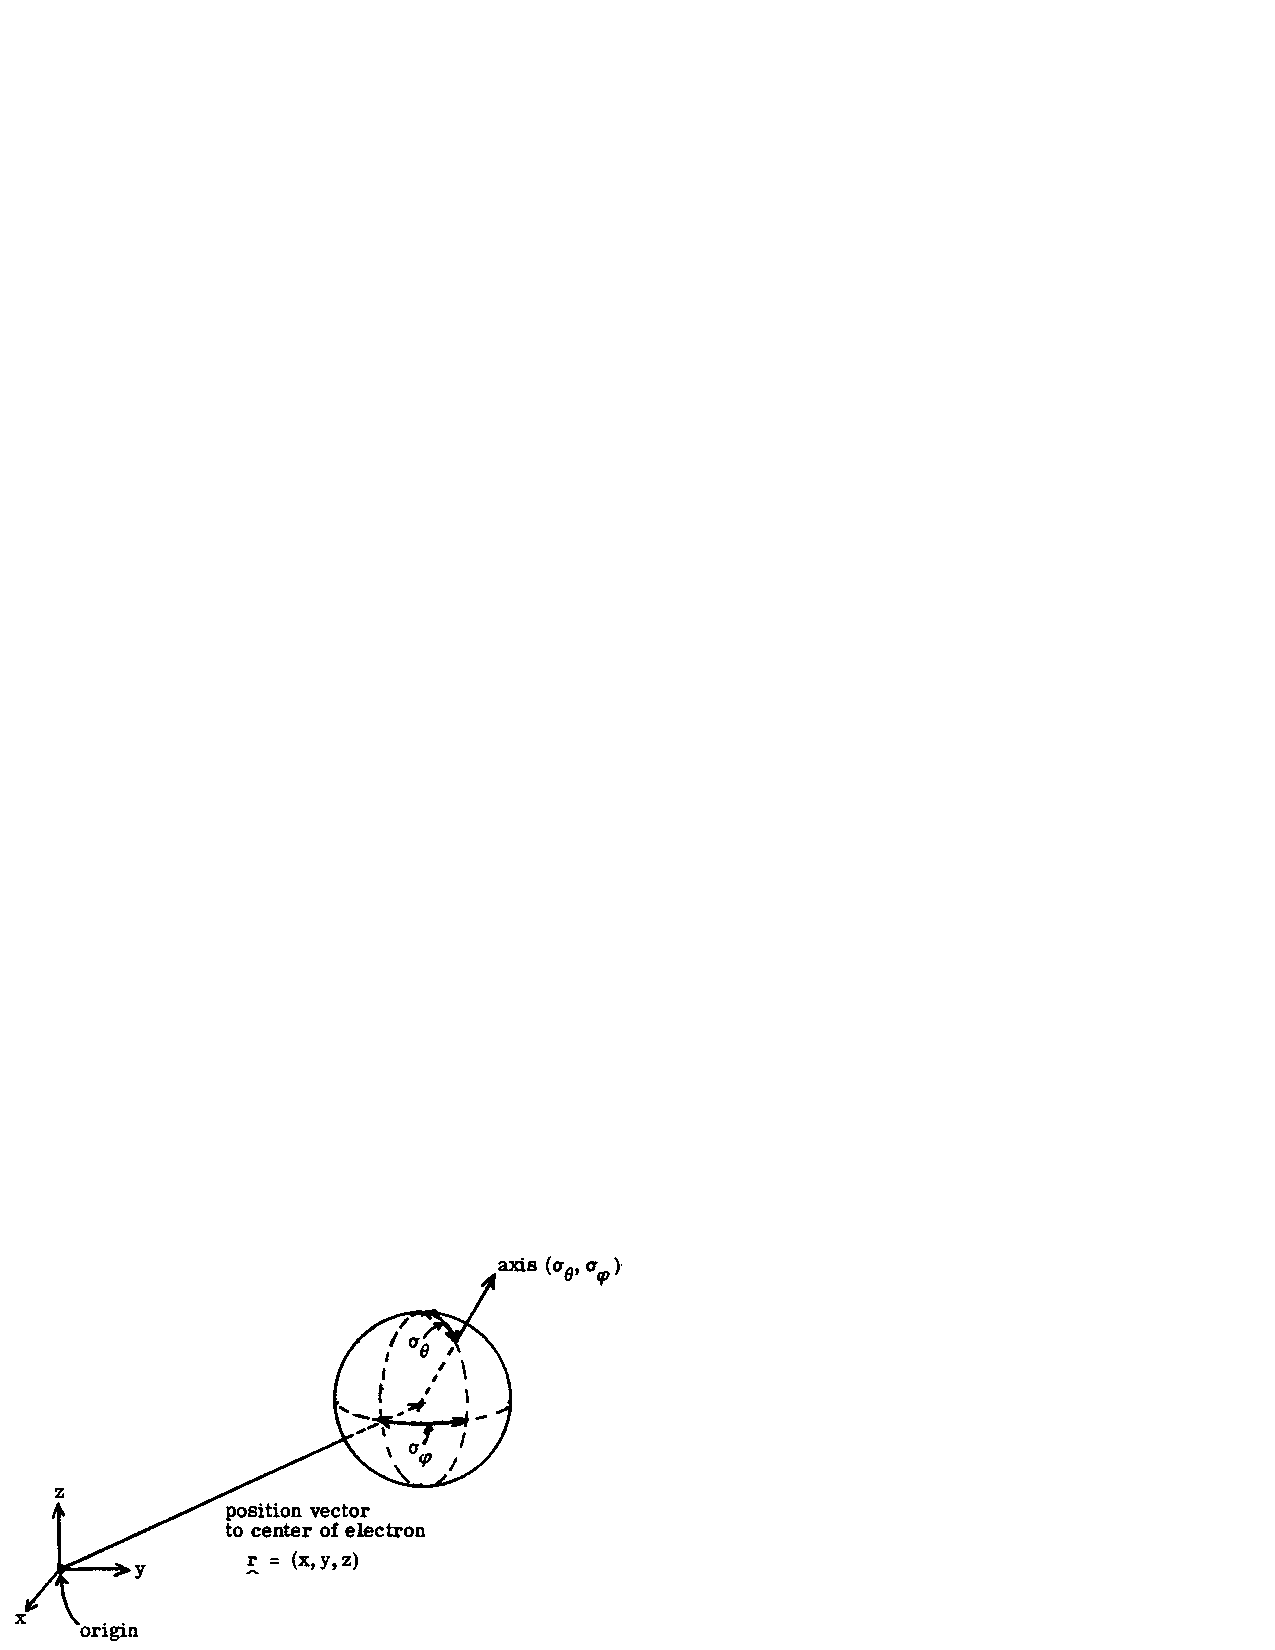
\includegraphics[scale=0.75]{fig4-1}
\caption{}
\label{fig4-01}
\end{figure}

So far, in this course, we have considered the electron to be a point particle
having mass $m$ and charge $-e$.  Thus, we described the electron wavefunction as
\begin{equation}
\varphi ( {\bf r} ) = \varphi ( x , y , z ) ,
\end{equation}
presuming that only the position of the electron need be given.
Imagine now that the electron has some finite size, say a small
sphere. Then we would need to specify, not only the position $x$, $y$,
and $z$ of the electron, but also the orientation of the sphere, say
$\sigma_v$, $\sigma_{\varphi}$, as indicated in Figure \ref{fig4-01}.
Thus, we would have to specify five coordinates in order to completely
describe the total wavefunction,
\begin{equation}
\psi ( x , y , z , \sigma_v , \sigma_{\varphi} ) .
\end{equation}
If the orientation is independent of the absolute position, the 
wavefunction will factor into two parts,
\begin{equation}
\varphi ( x , y , z , \sigma_v , \sigma_{\varphi} ) = \varphi ( x , y , 
z ) \chi ( \sigma_v , \sigma_{\varphi} ) = \varphi ( {\bf r} ) \chi ( 
\sigma )_ ,
\end{equation}
where, as usual, $\varphi$ is the probability amplitude of finding the
electron at some point $x, y, z$.  Here, ${\bf r}$ is symbolic for the
collection of coordinates $ x , y , z$, and $\sigma$ is symbolic for
the collection of coordinates $\sigma_v$, $\sigma_{\varphi}$.  The
other function, $\chi$ gives the probability amplitude of finding some
particular orientation $\sigma_v$, $\sigma_{\varphi}$ on the electron.
These orientation coordinates $\sigma_v$, $\sigma_{\varphi}$ would be
called \emph{internal coordinates}.

Imagine now that the electron is spinning about its axis with some angular
momentum $s$. Since the electron is charged, the spin would lead to a 
magnetic moment $\mu = \gamma s$. This magnetic momentum could be detected 
by its interaction with an external magnetic field, say in the $z$ 
direction,
\begin{equation}
\Delta E = - \mu_z B_z = - \gamma B_z s_z .
\end{equation}
Classically, $s_z$ could have any value from $s_z = +|s|$ to $s_z = - 
|s|$, where $|s|$ is the total angular
momentum.  Experimentally, the electron leads to only two values of $s_z$,
\begin{equation}
s_z = + {1 \over 2} \hbar
\label{chap4-eqno1}
\end{equation}
\begin{equation}
s_z = - {1 \over 2} \hbar
\label{chap4-eqno2}
\end{equation}
This description of the electron as a finite size charged sphere
should not be taken literally.  It is only to indicate how one might
think of the internal coordinates.  However, it is the case that the
electron does have an internal angular momentum (called \emph{spin})
which leads to a magnetic moment that can interact with external
magnetic fields. There are only two possible states for the internal
coordinates of the electron, up-spin (\ref{chap4-eqno1}), denoted as
$\alpha ( \sigma )$ and down-spin (\ref{chap4-eqno2}), denoted as
$\beta ( \sigma )$.  These two states, $\alpha$ and $\beta$ are
orthogonal, and normalized so that we write
\begin{equation}
\langle \alpha | \beta \rangle = 0
\end{equation}
\begin{equation}
\langle \alpha | \alpha \rangle = 1
\end{equation}
\begin{equation}
\langle \beta | \beta \rangle = 1
\end{equation}
where the integration is over the internal (spin) coordiantes.

Consider now, the product of spatial functions, hereafter called orbitals,
e.g., $\varphi_i$ and $\varphi_j$, and spin functions, e.g., $\alpha$ 
and $\beta$, to form spin orbitals such as
\begin{eqnarray}
\psi_{i \alpha} ( {\bf r} , \sigma ) &=& \varphi_i ( {\bf r} ) \alpha ( 
\sigma )\cr
\psi_{i \beta } &=& \varphi_i\beta\cr
\psi_{j \alpha} &=& \varphi_j\alpha\cr
\psi_{j \beta} &=& \varphi_j\beta
\end{eqnarray}
Then,
\begin{equation}
\langle \psi_{i \alpha} | \psi_{j \alpha} \rangle = \langle \varphi_i | 
\varphi_j \rangle \langle \alpha | \alpha \rangle = \langle \varphi_i | 
\varphi_j \rangle
\end{equation}
and
\begin{equation}
\langle \psi_{i \alpha} | \psi_{j \beta} \rangle = \langle \varphi_i | 
\varphi_j \rangle \langle \alpha | \beta \rangle = 0 .
\end{equation}
Thus, states with different spin are always orthogonal, independent of the 
relation between $\varphi_i$ and $\varphi_j$.  States with the same spin are 
orthonormal if the $\varphi_i$ are orthonormal.

Now consider the $\{ \varphi_i \}$ to be eigenstates of the Hamiltonian
\begin{equation}
H \varphi_i = E_i \varphi_i,
\end{equation}
where $H$ is independent of spin. There are actually terms in the
Hamiltonian that are dependent upon spin (e.g., spin-orbital
coupling).  These terms can usually be neglected in discussing the
chemistry of nontransition metals and are ignored here.

Then
\begin{equation}
H \psi_{i \alpha} = \left( H \varphi_i \right) \alpha = E_i \varphi_{i 
\alpha} = E_i \psi_{i \alpha}
\end{equation}
and
\begin{equation}
H \psi_{i \beta} = E_i \psi_{i \beta},
\end{equation}
so that there are two spin orbital eigenstates corresponding to each 
orbital eigenstate.  Thus, with spin there are twice as many states as 
without spin.  For example, the state of the $H$ atoms become $\psi_{1 s 
\alpha}$, and $\psi_{1 s \beta}$ with energy
\begin{equation}
E = - {1 \over 2} \left( {e^2 \over a_0} \right)
\end{equation}
$\psi_{2s \alpha}$, $\psi_{2s \beta}$, $\psi_{2 py \beta}$, $\psi_{2pz 
\alpha}$, $\psi_{2pz \beta}$, with energy
\begin{equation}
E = - {1 \over 8} \left( {e^2 \over a_0} \right)
\end{equation}
and $\psi_{3s \alpha}$, $\psi_{3s \beta}$, etc., with energy
\begin{equation}
E = - {1 \over 18} \left( {e^2 \over a_0} \right) ,
\end{equation}
etc.

In quantum mechanics, a state with total angular moment quantum number $L$
leads to a total of $2L + 1$ states having component along the $z$ axis of
\begin{equation}
M_L = + L , + L - 1 , + L - 2 ,\dots , -L + 1 , - L .
\end{equation}
A more proper review of angular momentum is given in Section
\ref{chap4-app-b}.  Thus, with $L = 1$ we obtain three states, 
$M_L = + 1, 0, - 1$. With $L = 1/2$ we obtain two states, $M_L = +
1/2$, and $-1/2$.  The spin of an electron has two possible states,
$M_S = + 1/2$ and $-1/2$, and we say that the electron has a spin of
\emph{one-half}.

\subsection{Two Electrons}

If $\Phi(1,2)$ is an eigenfunction of the two-electron Hamiltonian 
$H(1,2)$,
\begin{equation}
H(1,2) \Phi(1,2) = E \Phi(1,2) ,
\label{chap4-eqno3}
\end{equation}
the inclusion of electron spin leads to a total of four states,
\begin{equation}
\Psi_{\alpha \alpha} (1,2) = \Psi(1,2) \alpha ( 1 ) \alpha ( 2 )
\end{equation}
\begin{equation}
\Psi_{\alpha \beta} ( 1 , 2 ) = \Psi ( 1 , 2 ) \alpha ( 1 ) \beta ( 2 )
\end{equation}
\begin{equation}
\Psi_{\beta \alpha} ( 1 , 2 ) = \Psi ( 1 , 2 ) \beta ( 1 ) \alpha ( 2 )
\end{equation}
\begin{equation}
\Psi_{\beta\beta} ( 1 , 2 ) = \Psi ( 1 , 2 ) \beta ( 1 ) \beta ( 2 )
\end{equation}
all of which are eigenfunctions of $H$
\begin{equation}
H \Psi_{ij} = E \Psi_{ij} 
\label{chap4-eqno4}
\end{equation}
with the same energy. In Chapter 2 we found that since the Hamiltonian is
unchanged upon transposing the electrons,
\begin{equation}
H (1 , 2) = H ( 2 , 1),
\end{equation}
then its eigenstates (\ref{chap4-eqno3}) must each be either symmetric
or antisymmetric upon transposition, $\tau$,
\begin{equation}
\tau \Phi = \pm \Phi
\label{chap4-eqno5}
\end{equation}
Thus, for H$_2$,we found that the lowest two states have the form
\begin{equation}
\Phi_g ( 1 , 2 ) = \chi_l \chi_r + \chi_r \chi_l
\end{equation}
and
\begin{equation}
\Phi_u ( 1 , 2 ) = \chi_l \chi_r - \chi_r \chi_l ,
\end{equation}
which satisfy
\begin{equation}
\tau \Phi_g = + \Phi_g
\end{equation}
and
\begin{equation}
\tau \Phi_u = - \Phi_u
\end{equation}
Similarly, for He we found that the ground state was
\begin{equation}
\Phi ( 1 , 2 ) = \varphi_{1s} (1) \varphi_{1s} (2) ,
\end{equation}
which satisfies
\begin{equation}
\tau \Phi = + \Phi .
\end{equation}  

Including spin, the Hamiltonian remains rigorously symmetric under
interchange of the electrons, since the electrons are identical.  We
now must interchange both spatial and spin coordinates simultaneously,
denoting this as ${\bar \tau}$.  Thus, the spatial spin eigenstates
$\Psi_{ij}$ in (\ref{chap4-eqno4}) must also satisfy
\begin{equation}
{\bar \tau} \Psi_{ij} = \pm \Psi_{ij} 
\label{chap4-eqno6}
\end{equation}
Since
\begin{equation}
\Psi_{ij} = \Phi \chi_{ij} ,
\end{equation}
where $\chi_{ij}$ is a two-electron spin function, and since $\Phi$
satisfied (\ref{chap4-eqno5}), then (\ref{chap4-eqno6}) becomes
\begin{equation}
{\bar \tau} \Psi_{ij} = \left( {\bar \tau} \Phi \right) \left( {\bar 
\tau} \chi_{ij} \right) = ( \pm ) \Phi ( {\bar \tau} \chi_{ij} ) = ( 
\pm ) \Psi_{ij} = ( \pm ) \Phi \chi_{ij} .
\end{equation}
The $( \pm )$ in various terms indicates only that either + or $-$ may 
appear here, the $( \pm )$ of different terms need not be correlated.

Thus, we must have
\begin{equation}
{\bar \tau} \chi_{ij} = \pm \chi_{ij}
\label{chap4-eqno7}
\end{equation}
that is, the spin functions must be either symmetric or antisymmetric
under transposition of the electrons. But
\begin{equation}
{\bar \tau} \alpha \alpha = + \alpha \alpha ,
\end{equation}
\begin{equation}
{\bar \tau} \alpha \beta = \beta \alpha ,
\end{equation}
\begin{equation}
{\bar \tau} \beta \alpha = \alpha \beta
\end{equation}
\begin{equation}
{\bar \tau} \beta \beta = \beta \beta
\end{equation}
so that the $\alpha \beta$ and $\beta \alpha$ terms do not satisfy
(\ref{chap4-eqno7}).  Recombining spin terms, we get
\begin{equation}
^3\chi_{\alpha \alpha} = \alpha \alpha ,
\end{equation}
\begin{equation}
^3\chi_{\alpha \beta} = \left( \alpha \beta + \beta \alpha \right) ,
\end{equation}
\begin{equation}
^3\chi_{\beta \beta} = \beta \beta
\end{equation}
\begin{equation}
^1\chi_{\alpha \beta} = ( \alpha \beta - \beta \alpha ) ,
\end{equation}
where the three $^3\chi_{ij}$ terms are symmetric and the $^1\chi$ terms is 
antisymmetric, the notation will become clear momentarily.

\begin{table}
\caption{Permutational symmetries for wavefunctions of H$_2$ and He.}
\label{table4-01}

\begin{tabular}{cccccc}\\ \hline

& &\multicolumn{3}{c}{Permutation Symmetry} & Observed?\cr
& & Spatial & Spin & Total &\cr \hline
H$_2$ & $(\chi_l\chi_r + \chi_r\chi_l)(\alpha \alpha)$ & + & + & + & no\cr
& $(\chi_I\chi_r + \chi_r\chi_I)(\alpha \beta + \beta 
\alpha)$ & + & + & + & no\cr
& $(\chi_I\chi_r + \chi_r\chi_I)(\beta \beta )$ & + & + & + & no\cr
& $(\chi_I\chi_r + \chi_r\chi_I)(\alpha \beta - \beta 
\alpha)$ & + & $-$ & $-$ & yes\cr
& $(\chi_I\chi_r - \chi_r\chi_I)(\alpha \alpha)$ & $-$ & + & $-$ & yes\cr
& $(\chi_I\chi_r - \chi_r\chi_I)(\alpha \beta + \beta 
\alpha)$ & $-$ & + & $-$ & yes\cr
& $(\chi_I\chi_r - \chi_r\chi_l)(\beta \beta)$ & $-$ & + & $-$ & yes\cr
& $(\chi_I\chi_r - \chi_r\chi_I)(\alpha \beta - \beta 
\alpha)$ & $-$ & $-$ & + & no\cr
He & $(\varphi_{1s} \varphi_{1s} ) ( \alpha \alpha )$ & + & + & + & no\cr
& $( \varphi_{1s} \varphi_{1s} ) ( \alpha \beta + \beta \alpha )$ & + & + & + & 
no\cr
& $( \varphi_{1s} \varphi_{1s} ) ( \beta \beta )$ & + & + & + & no\cr
& $( \varphi_+{1s} \varphi_{1s} ) ( \alpha \beta - \beta 
\alpha )$ & + & $-$ & $-$ & yes\cr \hline
\end{tabular}
\end{table}

Combining the above results on spin and permutational symmetry, we
obtain the states of H$_2$ and He in Table \ref{table4-01}. As
expected, there are four possible spatial-spin states for each spatial
state, leading to a quadrupling of the states of the system, just as
the number of states for a one-electron system doubled.  In each case,
all four states are equally good, all being eignestates of the
Hamiltonian wit the same energy.  However, some of these states are
never observed. For two-electron systems, the only states that have
ever been observed are those that are permutationally antisymmetric,
\begin{equation}
{\bar \tau} \Psi = - \Psi .
\end{equation}
This fact, that only antisymmetric states are observed, is
incorporated into quantum mechanics by adding a new postulate called
the \emph{Pauli principle}, as will be discussed in the next section.

\section{The Pauli Principle}

In the previous section, we saw that for two electrons the identity of 
the electrons leads to the expectation that each eigenstates of $H$ has 
the symmetry
\begin{equation}
{\bar \tau} \Psi = \pm \Psi ,
\end{equation}
where ${\bar \tau}$ interchanges all coordinates, spatial and spin, of the 
two particles.  However, we noted that all experiments on electrons suggest 
that
\begin{equation}
{\bar \tau} \Psi = - \Psi
\end{equation}
is the only allowed permutational symmetry for electrons. Section
\ref{chap4-app-d} has some of the historical development leading to
these ideas. We incorporate these observations into quantum mechanics
with the following postulate.  The Pauli principle states that the
wavefunction for any system of electrons must change sign upon
interchange (transposition) of all coordinates (space and spin) of any
two electrons. This is a basic postulate of quantum mechanics, and is
justified by correct predictions for numerous systems.

To see what the Pauli Principle means, consider a simple two-electron 
wavefunction,
\begin{equation}
\Psi_A (1 , 2 ) = \psi_a (1) \psi_b (2) ,
\label{chap4-eqno8}
\end{equation}
where 1 symbolizes all spatial and spin coordinates of electron 1 and 2, 
the same for electron 2.

After interchanging the electrons, we get a new wavefunction,
\begin{equation}
\Psi_B (1,2) = \Psi_A (2,1) = \psi_b(1) \psi_a (2).
\label{chap4-eqno9}
\end{equation}
The Pauli principle states that
\begin{equation}
\Psi_B (1,2) = - \Psi_A (1,2)
\end{equation}
and hence, that
\begin{equation}
\psi_b (1) \psi_a (2)  = \psi_a (1) \psi_b (2) .
\end{equation}
This is obviously not true, and, thus, the simple wavefunction
(\ref{chap4-eqno8}) is not acceptable for describing electrons.

However, it is easy to fix up a suitable wavefunction by subtracting
(\ref{chap4-eqno9}) from (\ref{chap4-eqno8}),
\begin{equation}
\Psi_C (1,2) = \Psi_A (1,2) - \Psi_A (2,1) = \psi_a (1) \psi_b (2) - 
\psi_b (1) \psi_a (2).
\label{chap4-eqno10}
\end{equation}
Thus, starting with (10) and interchanging electrons, leads to
\begin{eqnarray}
\Psi_C (2,1) &=& \psi_a (2) \psi_b (1) - \psi_b (2) \psi_a (1)\cr
&=& \psi_b (1) \psi_a (2) - \psi_a (1) \psi_b (2)\cr
&=& - \psi_a (1) \psi_b (2) + \psi_b (1) \psi_a (2)\cr
&=& - \Psi_C (1,2),
\end{eqnarray}
so that the wavefunction (\ref{chap4-eqno10}) does indeed satisfy the
Pauli principle.

For convenience in describing wavefunctions such as
(\ref{chap4-eqno10}), we will define the antisymmetrizer ${\cal A}$
\begin{equation}
{\cal A} \psi_a (1) \psi_b (2) = \psi_a (1) \psi_b (2) - \psi_b (1) 
\psi_a (2),
\label{chap4-eqno11}
\end{equation}
which takes a spin orbital product and converts it into a wavefunction
satisfying the Pauli principle.  Now let us consider some simple
cases.

\subsection{Identical Spin Orbitals}

Assume that $\psi_b = \psi_a$.  In this case, the wavefunction
(\ref{chap4-eqno10}) and (\ref{chap4-eqno11}) becomes
\begin{equation}
\psi_a (1) \psi_a (2) - \psi_a (1) \psi_a (2) = 0.
\end{equation}
Therefore, the Pauli principle says that we cannot have two electrons in 
the same spin orbital.

\subsection{Orthogonality of Spin Orbitals}

Consider a case where $\psi_a$ and $\psi_b$ are orthogonal,
\begin{equation}
\langle \psi_a | \psi_b \rangle = 0
\end{equation}
and define a new function
\begin{equation}
\psi_c = \psi_b + \lambda \psi_a ,
\end{equation}
where $\lambda \not= 0$, so that $\psi_c$ is not orthogonal to $\psi_a$,
\begin{equation}
\langle \psi_a | \psi_c \rangle = \langle \psi_a | \psi_b \rangle + \lambda 
\langle \psi_a | \psi_a \rangle = 0 + \lambda = \lambda \not= 0 .
\end{equation}
Forming a new wavefunction, using $\psi_a$ and $\psi_c$ V), we obtain
\begin{eqnarray}
\psi_a (1) \psi_c (2) - \psi_c (1) \psi_a (2) &= \psi_a \psi_b + \lambda 
\psi_a \psi_a - \psi_b \psi_a - \lambda \psi_a \psi_a\cr
&= \psi_a \psi_b - \psi_a \psi_a .\cr
\end{eqnarray}
Because of the Pauli principle, the wavefunction with partially
overlapping spin orbitals $\psi_a$ and $\psi_b$ is identical to the
waverfunction in which these spin orbitals are orthogonal.
Consequently, we say that the Pauli principle leads to orthogonality
of spin orbitals.  Since the spin orbitals are normalized, we can
require that the spin orbitals of antisymmetric wavefunctions
(\ref{chap4-eqno10}) and (\ref{chap4-eqno11}), be orthonormal,
\begin{equation}
\langle \psi_i | \psi_j \rangle = \delta_{ij} .
\label{chap4-eqno12}
\end{equation}

\subsection{Nonuniqueness}

Starting with the wavefunctions (\ref{chap4-eqno10}) and
(\ref{chap4-eqno11}), consider the new wavefunction
\begin{equation}
\Psi_2 = {\cal A} \bar{\psi}_a \bar{\psi}_b  
  = \bar{\psi}_a \bar{\psi}_b - \bar{\psi}_b \bar{\psi}_a, 
\label{chap4-eqno13}
\end{equation}
where
\begin{equation}
\bar{\psi}_a = \cos \theta \psi_a + \sin \theta \psi_b
\label{chap4-eqno14a}
\end{equation}
and
\begin{equation}
\bar{\psi}_b = - \sin \theta \psi_a + \cos \theta \psi_b .
\label{chap4-eqno14b}
\end{equation}
If $\psi_a$ and $\psi_b$ are orthonormal, (\ref{chap4-eqno12}), then
the new orbitals $\bar{\psi}_a$ and $\bar{\psi}_b$ are also
orthonormal,
\begin{equation}
\langle \bar{\Psi}_i \vert \bar{\Psi}_j \rangle = \delta_{ij} .
\end{equation}
Substituting (\ref{chap4-eqno14a})--(\ref{chap4-eqno14b}) into
(\ref{chap4-eqno13}) leads to
\begin{eqnarray}
\Psi_2 &=& -\sin\theta\cos\theta {\cal A} \psi_a \psi_a 
   + \sin\theta\cos\theta {\cal A} \psi_b \psi_b \\
  &&+ \cos^2 \theta {\cal A} \psi_a\psi_b - \sin^2 \theta {\cal A}
   \psi_b \psi_a \\
  &=& {\cal A} \psi_a\psi_b = \Psi_1
\end{eqnarray}
or
\begin{equation}
{\cal A} \bar{\psi}_a \bar{\psi}_b = {\cal A} \psi_a \psi_b .
\end{equation}
Thus, given an antisymmetrized wavefunction written in terms of spin
orbitals $\psi_a$ and $\psi_b$, this wavefunction is unchanged upon
recombining the spin orbitals; the wavefunction retains
orthonormality.  The Pauli principle states that only the
two-dimensional space spanned by $\psi_a$ and $\psi_b$ is significant,
but not the particular axis or basis functions used to describe this
space.

\subsection{Summary for Two Electrons}

Starting with two spin orbitals $\psi_a$ and $\psi_b$, one could construct 
four possible wavefunctions,
\begin{equation}
\psi_a (1) \psi_a (2)
\end{equation}
\begin{equation}
\psi_a (1) \psi_b (2)
\end{equation}
\begin{equation}
\psi_b (1) \psi_a (2)
\end{equation}
\begin{equation}
\psi_b (1) \psi_b (2) .
\end{equation}
Of these four possibilities, only the following combination of the second 
and third functions
\begin{equation}
\psi_a (1) \psi_b (2) = \psi_a (1) \psi_b (2) - \psi_b (1) \psi_a 
(2)
\label{chap4-eqno15}
\end{equation}
are allowed by the Pauli principle.

For convenience in writing such wavefunctions, we define the
antisymmetrizer ${\cal A}$, so that ${\cal A} \psi_a \psi_b$ is always
understood to denote $\psi_a \psi_b - \psi_b \psi_a$.  If the two spin
orbitals are identical, the wavefunction (\ref{chap4-eqno15}) is zero
and, indeed, the spin orbitals can be taken as orthogonal without
affecting the wavefunction.  Moreover, the spin orbitals $\psi_a$ and
$\psi_b$ can be recombined, retaining orthonormality, without changing
the wavefunction.  For the antisymmetrized wavefunction
(\ref{chap4-eqno15}), any overlap between the spinorbitals gets
zapped, deleted, by the antisymmetrizer; hence, the spin orbitals can
be taken as orthogonal, with no restriction.

\subsection{Determinants}

There is a simple way to use determinants in writing wavefunctions 
satisfying the Pauli principle.  The determinant is defined as
\begin{equation}
\left| \matrix{a & b\cr
c & d\cr}\right| = ad - bc
\end{equation}
and
\begin{equation}\left| \matrix{ a & b & c\cr
d & e & f\cr
g & h & i\cr}\right| = aei + bfg + chd - ceg - bdi - ahf
\end{equation}
etc.  For matrices of orders 2 and 3, the determinant is most rapidlly 
calculated by assigning a $+1$ coefficient for products arising from 
multiplying along the downward diagonals, including parallel shifted 
diagonals, and assigning a $-1$ coefficient for
products arising from multiplying along upward diagonals.  The general 
definition is
\begin{equation}
\det \left[ a_{11} a_{12} \cdots a_{nn} \right] = \sum_{ij 
\cdots \omega} \epsilon_{ij \cdots \omega} a_{1i} 
a_{2j} \cdots a_{n \omega} ,
\end{equation}
where $\epsilon_{ij \cdots \omega} = 0$, unless all indices are
different, say $\epsilon_{ij \cdots \omega} = +1$ when $ij \cdots
\omega$ is an even permutation of $12 \cdots n$, and $\epsilon_{ij
\cdots \omega} = -1$ when $ij \cdots \omega$ is an odd permutation of
$12 \cdots n$.  An odd permutation is one that is constructed from an
odd number of transpositions, and an even permutation is one that is
constructed from an even number of transpositions.  Thus, the
determinant automatically changes sign upon interchange of any two
rows or columns.

Important properties of a determinant are:
\begin{enumerate}
\item The determinant changes sign upon interchange of any two rows or
any two columns, e.g.,
\begin{equation}
\left| \matrix{b & c\cr
d & e\cr} \right| = bd - ad = - \left| \matrix{a & b \cr
c & d\cr} \right|.
\end{equation}
\item The determinant is zero, if any two columns, or any two rows,
are identical, e.g.,
\begin{equation}
\left| \matrix{a & a\cr
c & c\cr} \right| = ac - ac = 0 .
\end{equation}
\item Adding some amount of any one column to any other column, leaves
the determinant unchanged,
\begin{equation}
\left| \matrix{a & b+ \lambda a\cr
c & d+ \lambda c\cr} \right| = a(d+ \lambda c ) - ( b + \lambda a ) c = 
ad + \lambda ac - bd - \lambda ac = \left| \matrix{a & b \cr
d & d \cr} \right|
\end{equation}
(the same is true for rows).  Thus, each row can be made as orthogonal 
to each other row without changing the determinant.
\end{enumerate}

The wavefunction (\ref{chap4-eqno15}) can be written as a determinant,
as follows
\begin{equation}
\left| \matrix{\psi_a (1) & \psi_b (1)\cr
\psi_a (2) & \psi_b(2)\cr} \right| = \psi_a (1) \psi_b (2) - \psi_b (1) 
\psi_a (2) = {\cal A} \psi_a (1) \psi_b (2)
\end{equation}
where the antisymmetrizer ${\cal A}$ can be referred to as the 
\emph{determinant operator}.

Similarly, starting with the $3! = 6$ product wavefunctions,
\begin{equation}
\psi_a (1) \psi_b (2) \psi_c (3)
\end{equation}
the only combination satisfying the Pauli principle is
\begin{eqnarray}
\Psi (1,2,3) &=& \mathcal{A}\psi_a (1) \psi_b (2) \psi_c (3)\\
    &=& \left[ \psi_a \psi_b \psi_c + \psi_b \psi_c \psi_a + \psi_c 
\psi_a \psi_b - \psi_b \psi_a \psi_c - \psi_c \psi_b \psi_a - \psi_a 
\psi_c \psi_b \right]\\
   &=& \left| \matrix{\psi_a (1) & \psi_b (1) & \psi_c (1)\cr
\psi_a (2) & \psi_b (2) & \psi_c (2)\cr
\psi_a (3) & \psi_b (3) & \psi_c (3)\cr} \right|
\label{chap4-eqno16}
\end{eqnarray}
For example, interchanging electrons 1 and 3, leads to
\begin{eqnarray}
\Psi (3,2,1) &=& \left[ \psi_c \psi_b \psi_a + \psi_a \psi_c \psi_b + 
\psi_b \psi_a \psi_c - \psi_c \psi_a \psi_b - \psi_a \psi_b \psi_c - 
\psi_b \psi_c \psi_a \right]\\
&=& - \psi_a \psi_b \psi_c - \psi_b \psi_c \psi_a - \psi_c \psi_a \psi_b + 
\psi_b \psi_a \psi_c + \psi_c \psi_b \psi_a + \psi_a \psi_c \psi_b\\
&=& - \Psi (1 , 2, 3 ).
\end{eqnarray}
Note also, from the properties of determinants, that interchange of
any two columns of (\ref{chap4-eqno16}) (i.e. interchanging two spin
orbitals) merely changes the sign of the wavefunction so that
\begin{equation}
{\cal A} \psi_b \psi_a \psi_c = -{\cal A} \psi_a \psi_b \psi_c .
\end{equation}

Using the properties of the determinant, one can show that:
\begin{enumerate}
\item ${\cal A} \psi_a \psi_b \psi_c \cdots$ 
changes sign upon interchange of any pair of electrons, thus the Pauli
principle is always satisfied.
\item ${\cal A} \psi_a \psi_b \psi_c \cdots = 0$ 
if any two spin orbitals are equal (e.g. ${\cal A} \psi_a \psi_a
\psi_c = 0$).  
\item All orbitals in ${\cal A} \psi_a \psi_b \psi_c$ can be taken as
orthogonal with no restrictions.  Thus, we take $\langle \psi_i | \psi_j 
\rangle = \delta_{ij}$.  
\item Interchange of any two spin orbitals of 
${\cal A} \psi_a \psi_b \psi_c \cdots$ 
merely changes the sign of the wavefunction.  Thus, any permutation of the 
spin orbitals leads back to the original wavefunction, or else changes the 
sign.   Since the sign of the total wavefunction has no significance, the 
order of the spin orbitals in ${\cal A} \psi_a \psi_b \psi_c \cdots$ 
is of no significance.  
\item We may take any recombination of the $\psi_i$, preferring
orthonormality to obtain ${\cal A} \bar{\psi}_a \bar{\psi}_b
\bar{\psi}_c \cdots = {\cal A} \psi_a \psi_b \psi_c \cdot \cdot
\cdot$.
\end{enumerate}

For an $N$-electron system, there are $N!$ possible product terms, such as
\begin{equation}
\psi_a (1) \psi_b (2)\cdots\psi_z (N) .
\end{equation}
Of these, there is one combination that satisfies the Pauli principle.  
This combination can be written as an $N$ by $N$ determinant
\begin{equation}
\det\psi_a (1) \psi_b (2) \cdots \psi_z (N) ,
\end{equation}
where the spin orbitals are orthonormal
\begin{equation}
\langle \psi_i \vert \psi_j \rangle = \delta_{ij} .
\end{equation}
Such determinants of functions are referred to in the mathematical
literature as St\"ackel determinants.  They were first used to
describe electronic wavefunctions by Heisenberg and were popularized
by J. L.  Slater \cite{chap4-ref1}. They are often referred to as
\emph{Slater determinants}.

For $N$ noninteracting but identical particles, there would be $N!$ 
possible states, all with the same energy.  Of these, only one is allowed 
by quantum mechanics.  In developing statistical mechanics, the famous 
engineer J. W. Gibbs, realized that use of $N!$ factor led to ridiculous 
entropies and arbitrarily just divided the total number of
states by $N!$.  He got the right answer but missed a golden opportunity 
to invent quantum mechanics before the physicists stumbled into it.

\subsection{More on Spins for Two Electrons}

Defining the total $M_s$ quantum number for a spin function, as the sum 
of the $M_s$ numbers for each electron, leads to
\begin{eqnarray}
\left. \matrix{\alpha\alpha & M_s = +1\cr
\alpha \beta + \beta \alpha & M_s = 0\cr
\beta \beta & M_s = -1\cr}\right\} s = 1\cr
\end{eqnarray}
\begin{equation}
\left. \alpha \beta - \beta \alpha ~~ M_s = 0\right\} s = 0.
\end{equation}
The three states of the triplet have $M_S = +1, 0, - 1$, and we refer
to this as the \emph{spin-one states} ($S = 1$).  Whereas the singlet
state has only $M_S = 0$, we refer to this as the \emph{spin-zero
states} ($S=0$).  Spin states are discussed more carefully in a
following section.

\subsection{Noninteracting Particles}

Consider, for the moment, a simple system in which the electrons do not 
interact, say one electron in California and the other on the moon.  The 
Hamiltonian of the system is
\begin{equation}
H(1,2) = h(1) + h(2),
\end{equation}
and if $\psi_a$ and $\psi_b$ are eigenstates of $h$,
\begin{equation}
h \psi_a = \epsilon_a \psi_a
\end{equation}
and
\begin{equation}
h \psi_b = \epsilon_b \psi_b ,
\end{equation}
then either produce wavefunction is an eigenfunction of $H$
\begin{equation}
H \psi_a \psi_b = \left( \epsilon_a + \epsilon_b \right) \psi_a \psi_b
\end{equation}
and
\begin{equation}
H \psi_b \psi_a = \left( \epsilon_a + \epsilon_b \right) \psi_b \psi_a .
\end{equation}
However, the Pauli principle says that only the wavefunction
(\ref{chap4-eqno15})
\begin{equation}
\psi = \psi_a \psi_b - \psi_b \psi_a
\end{equation}
is allowed.  Thus, even electrons 200,000 miles apart have a
phase relation connecting them.  Quantum mechanics is
stranger than fiction!

\section{Spin for Two or More Electrons}

\subsection{Two Electrons}
    
Because of the Pauli principle, only one spin state is consistent with the
symmetric spatial wavefunction,
\begin{equation}
\left( \varphi_a \varphi_b + \varphi_b \varphi_a \right) \left( \alpha 
\beta - \beta \alpha \right)
\label{chap4-eqno17}
\end{equation}
and, consequently, this is called a \emph{singlet state}.  On the
other hand, three spin states are allowed for an antisymmetric spatial
wavefunction,
\begin{equation}
\left( \varphi_a \varphi_b - \varphi_b \varphi_a \right)\left( \alpha 
\alpha \right)
\label{chap4-eqno18a}
\end{equation}
\begin{equation}
\left( \varphi_a \varphi_b - \varphi_b \varphi_a \right)\left( \alpha 
\beta + \beta \alpha \right)
\label{chap4-eqno18b}
\end{equation}
\begin{equation}
\left( \varphi_a \varphi_b - \varphi_b \varphi_a \right)\left( \beta 
\beta \right)
\label{chap4-eqno18c}
\end{equation}
and these are collectively referred to as a \emph{triplet state}.

Since the energy expression does not depend upon spin, the energies of
the allowed wavefunctions (\ref{chap4-eqno17}) and
(\ref{chap4-eqno18a})--(\ref{chap4-eqno18c}) are the same as for the
forbidden states,
\begin{equation}
\left( \varphi_a \varphi_b + \varphi_b \varphi_a \right)\left( \alpha 
\alpha \right)
\end{equation}
\begin{equation}
\left( \varphi_a \varphi_b + \varphi_b \varphi_a \right)\left( \alpha 
\beta + \beta \alpha \right)
\end{equation}
\begin{equation}
\left( \varphi_a \varphi_b + \varphi_b \varphi_a \right)\left( \beta 
\beta \right)
\end{equation}
\begin{equation}
\left( \varphi_a \varphi_b - \varphi_b \varphi_a \right) \left( \alpha 
\beta - \beta \alpha \right) ,
\label{chap4-eqno19}
\end{equation}
respectively.  However, because of the Pauli principle, only
(\ref{chap4-eqno17})--(\ref{chap4-eqno18c}) are allowed, leading to
a correlation between spatial symmetry (and hence, energy) and spin.
Thus, if $\varphi_a$ and $\varphi_b$ are the $\chi_l$ and $\chi_r$
orbitals of H$_2$, state 1 is better, leading to the singlet spin
state.  In this case, we say that bonding electrons prefer to have
their spins aligned antiparallel.  On the other hand, if $\varphi_a$
and $\varphi_b$ are the $\varphi_g$ and $\varphi_u$ orbitals of the
excited state of H$_2$, then state 2 is better and we say that
electrons in orthogonal orbitals prefer to have their spin aligned
parallel.  Of course the spin has nothing to do with the energy, but
such descriptions do serve to keep track of the spatial symmetries
that do determine energy.

Since the three spin functions in (\ref{chap4-eqno18a})
--(\ref{chap4-eqno18c}) all lead to the
same energy, it is sufficient to consider just one.  We will always
use the maximum value of $M_S$, namely, $\alpha \alpha$ for $S = 1$
and, $\alpha\beta - \beta\alpha$ for $S = 0$.  Thus,
(\ref{chap4-eqno17}) becomes
\begin{eqnarray}
\left( \varphi_a \varphi_b - \varphi_b \varphi_a \right) \alpha \alpha &=& 
\left[ \varphi_a (1) \varphi_b (2) - \varphi_b (1) \varphi_a (2) \right] 
\alpha ( 1 ) \alpha (2)\cr
&=& \left( \varphi_a \alpha \right) \left( \varphi_b \alpha \right) - 
\left( \varphi_b \alpha \right) \left( \varphi_a \alpha \right)\cr
&=& {\cal A} \left[ \left( \varphi_a \alpha \right) \left( \varphi_b 
\alpha \right) \right]
\end{eqnarray}
On the other hand, the wavefunction (\ref{chap4-eqno19}) requires two
determinants,
\begin{eqnarray}
\left( \varphi_a \varphi_b + \varphi_b \varphi_a \right) \left( \alpha 
\beta - \beta \alpha \right) &=& {\cal A} \left( \varphi_a \varphi_b + 
\varphi_b \varphi_a \right) \alpha \beta\cr
&=&{\cal A} \left( \varphi_a \alpha \right) \left( \varphi_b \beta 
\right) + {\cal A} \left( \varphi_b \alpha \right) \left( \varphi_a \beta 
\right)\cr
&=& {\cal A} \left( \varphi_a \varphi_b \right) \left( \alpha \beta - \beta 
\alpha \right).
\end{eqnarray}

\subsection{Three Electrons}

For three electrons, there are eight spin functions, $\alpha \alpha 
\alpha$, $\alpha \alpha \beta$, $\alpha \beta \alpha$, $\beta \alpha 
\alpha$, $\alpha \beta \beta$, $\beta \alpha \beta$, $\beta \beta \alpha$, 
and $\beta \beta \beta$.  You should check to see that all eight 
functions are orthogonal.  Combining these into proper spin functions, leads to
\begin{equation}
\left. \matrix{\alpha \alpha \alpha & M_S + {3 \over 2}\cr
\alpha \alpha \beta + \alpha \beta \alpha & M_S + {1 \over 2}\cr
\alpha \beta \beta + \beta \alpha \beta + \beta \beta \alpha & M_S = - {1 
\over 2}\cr
\beta \beta \beta & M_S = - {3 \over 2}\cr}\right\} s + {3 \over 2} ~ 
{\rm quartet}
\end{equation}
\begin{equation}
\left. \matrix{(\alpha \beta - \beta \alpha)\alpha & M_s = {1 \over 2}\cr
(\alpha \beta - \beta \alpha ) \beta & M_s = - {1 \over 2}\cr}\right\} s = 
{1 \over 2} ~ {\rm doublet}
\end{equation}
\begin{equation}
\left. \matrix{ 2 ( \alpha \alpha ) \beta - ( \alpha \beta + \beta 
\alpha ) \alpha & M_S = {1 \over 2}\cr
( \alpha \beta + \beta \alpha ) \beta - 2 ( \beta \beta ) \alpha & M_S = - 
{1 \over 2}\cr}\right\} s = {1 \over 2} ~ {\rm doublet}
\end{equation}
The particular combinations involved here, for $M_s = 1/2$ and $M_S = - 
1/2$ are of no concern here.  In discussing the $S = 3/2$ or quartet, it is
sufficient to consider the $M_S = 3/2$ function of $\alpha(l)\alpha(2)\alpha(3)$.

\subsection{Spin States for N Electrons}

Given two choices, $\alpha$ and $\beta$, for the spin of each electron, 
there are $2N$ possible spin functions for an $N$-electron system. These 
functions are most conveniently discussed using the theory of angular 
momentum.  In this course, we make little explicit use of angular momentum 
theory.  However, the terminology incorporates aspects of this theory; 
hence, some discussion is appropriate.

Section \ref{chap4-app-b} contains a review of the formalism. The
results (relevant here) are the following.  A set of $2S + 1$ states,
\begin{equation}
\chi_{S,S} , \chi_{S,S-1} , \cdots , \chi_{S,-S}
\label{chap4-eqno20}
\end{equation}
is said to be an angular momentum $S$ state if
\begin{equation}
\hat{S}^2 \chi_{S,M} = S(S + 1) \chi_{S,M}
\end{equation}
and
\begin{equation}
\hat{S}_z \chi_{S,M} = M \chi_{S,M}
\end{equation}
where $\hat{S}^2$ and $\hat{S}_z$ are referred to as the total angular 
momentum operator and the angular momentum projection operator.  The 
numbers $S$ and $M$  must be integers or half-integers, leading to the 
following possible cases.  For singlet
\begin{equation}
S = 0 , M = 0
\end{equation}
for doublet
\begin{equation}
S = {1 \over 2} , M = \pm {1 \over 2}
\end{equation}
for triplet
\begin{equation}
S = 1 , M = 0, \pm 1
\end{equation}
for quartet
\begin{equation}
S = {3 \over 2} , M = \pm {1 \over 2} , \pm {3 \over 2}
\end{equation}
etc.  Since the Hamiltonian does not depend on spin, no magnetic
field, the $2S +1$ states in (\ref{chap4-eqno20}) all have the same
energy.  The states of $\chi_{S,M}$ with the same $S$ but different
$M$, are related by the raising and lowering operators, $\hat{S}^+$
and $\hat{S}^-$,
\begin{equation}
\hat{S}^+ \chi_{S,M} = \sqrt{S(S+1) - M_S (M_S + 1) \chi_{S,M+1}}
\label{chap4-eqno21a}
\end{equation}
\begin{equation}
\hat{S}^- \chi_{S,M+1} = \sqrt{S(S+1) - M_S (M_S + 1) \chi_{S,M}}.
\label{chap4-eqno21b}
\end{equation}
Thus, in particular,
\begin{equation}
\hat{S}^+ \chi_{S,S} = 0
\label{chap4-eqno22a}
\end{equation}
\begin{equation}
\hat{S}^- \chi_{S,-S} = 0.
\label{chap4-eqno22b}
\end{equation}
A convenient test for whether a function is a spin eigenfunction, is
as follows, using (\ref{chap4-eqno22a})--(\ref{chap4-eqno22b}).  If
\begin{equation}
\hat{S}_z \psi_M = M \psi_M
\end{equation}
and
\begin{equation}
\hat{S}^+ \psi_M = 0,
\end{equation}
then $\psi_M$ is an angular momentum state with $M = S$.

\subsubsection{One Electron}

Applying these properties to the one-electron case, $S = 1/2$, and $M = 
\pm 1/2$, leads to
\begin{equation}
\hat{s}_z \alpha = {1 \over 2} \alpha
\end{equation}
\begin{equation}
\hat{s}_z \beta = - {1 \over 2} \beta
\end{equation}
\begin{equation}
\hat{s}^2 \alpha = s ( s + 1 ) \alpha = {3 \over 4} \alpha
\end{equation}
\begin{equation}
\hat{s}^2 \beta = s ( s + 1 ) \beta = {3 \over 4} \beta
\end{equation}
where $s = 1/2$.  From (\ref{chap4-eqno21a})--(\ref{chap4-eqno21b})
\begin{equation}
\hat{s}^+ \alpha = 0
\end{equation}
\begin{equation}
\hat{s}^- \alpha = \beta
\end{equation}
\begin{equation}
\hat{s}^+ \beta = \alpha
\end{equation}
\begin{equation}
\hat{s}^- \beta = 0 .
\end{equation}
The one electron spin functions are orthonormal, that is
\begin{eqnarray}
\langle \alpha | \beta \rangle &= 0\cr
\langle \alpha | \alpha \rangle &= 1\cr
\langle \beta | \beta \rangle &= 1.\cr
%
\label{chap4-eqno23}
\end{eqnarray}

\subsubsection{Two Electrons}

With two electrons, we define the spin operators as
\begin{eqnarray}
\hat{S}_z &= \hat{s}_z (1) + \hat{s}_z (2)\cr
\hat{S}^+ &= \hat{s}^+ (1) + \hat{s}^+ (2)\cr
\hat{S}^- &= \hat{s}^- (1) + \hat{s}^- (2)\cr
\end{eqnarray}
and
\begin{equation}
\hat{S}_2 = \hat{S}^2_x + \hat{S}^2_y + \hat{S}^2_z .
\end{equation}
Applying the theory leads two-electron spin eigenfunctions of the form
\begin{equation}
S = 1: \left\{ \matrix{\chi_{11} = \alpha \alpha &\cr
\chi_{10} = {1 \over \sqrt{2}} (\alpha \beta + \beta \alpha ) &\cr
\chi_{1{\bar 1}} = \beta \beta &\cr}\right.
\label{chap4-eqno24}
\end{equation}
\begin{equation}
S = 0 : \chi_{00} = {1 \over \sqrt{2}} ( \alpha \beta - \beta \alpha 
)
\label{chap4-eqno25}
\end{equation}
Using the orthogonality of the one-electron spin functions
(\ref{chap4-eqno23}) we see that the four two-electron functions
(\ref{chap4-eqno24}) and (\ref{chap4-eqno25}) are orthonormal.  Since
$\hat{S}^+ \chi_{11} = 0$ and $\hat{S}^+ \chi_{00} = 0$, we see from
(\ref{chap4-eqno22a})--(\ref{chap4-eqno22b}) that these are spin
eigenfunctions with $S = 1$ and $S = 0$, respectively.  Since
\begin{equation}
\hat{S}^- \chi_{11} = \sqrt{2} \chi_{10}
\end{equation}
and
\begin{equation}
\hat{S}^- \chi_{10} = \sqrt{2} \chi_{1 \bar{1}} ,
\end{equation}
we find that $\chi_{10}$ and $\chi_{1 \bar{1}}$ are also $S = 1$ 
functions.

As derived in Section 4.3, from the Pauli principle, a triplet spin 
function (symmetric) such as $\alpha \alpha$ of (\ref{chap4-eqno24}) must go with an 
antisymmetric spatial function such as 
\begin{equation}
\varphi_a \varphi_b - \varphi_b \varphi_a ,
\label{chap4-eqno26}
\end{equation}
while a single spin function (anitsymmetric) such as $( \alpha \beta -
\beta \alpha )$ of (\ref{chap4-eqno25}) must go with a symmetric
spatial function such as
\begin{equation}
\varphi_a \varphi_b + \varphi_b \varphi_a
\label{chap4-eqno27}
\end{equation}
These permutational symmetries of wavefunctions are sometimes
illustrated by diagrams as in (\ref{chap4-eqno26}) and
(\ref{chap4-eqno27}), where orbitals in the same row are symmetrical
(permutationally), while orbitals in the same column are
antisymmetric.

In Chapter 3 we used the nodal theorem to show that the ground state of any 
two-electron system must have a symmetric spatial function.  Thus, because 
of the Pauli principle the ground state of any two-electron system must be 
a singlet spin state.

\subsubsection{Many Electrons}

Section \ref{chap4-app-c} shows how to construct spin eigenfunctions
for systems with more electrons.  An understanding of such functions
is important for discussing the states of transition metal systems but
will be deferred for now.  We will instead consider the spin
properties of some Slater determinant wavefunctions.

Consider first
\begin{equation}
\Psi_{11} = {\cal A} \left( \varphi_a \alpha \right) \left( \varphi_b \alpha 
\right).
\label{chap4-eqno28}
\end{equation}
Since
\begin{equation}
\hat{S}_x \Psi_{11} = \left( {1 \over 2} + {1 \over 2} \right) \Psi_{11} = 
\Psi_{11}
\end{equation}
and
\begin{equation}
\hat{S}^+ \Psi_{11} = 0 ,
\end{equation}
we see that $\Psi_{11}$ has $S = 1$ and $M = 1$.  This, of course, is 
obvious since expanding $\Psi_{11}$ leads to
\begin{equation}
\Psi_{11} = \left( \varphi_a \alpha \right) \left( \varphi_b \alpha \right) - 
\left( \varphi_b \alpha \right) \left( \varphi_a \alpha \right) = \left( 
\varphi_a \varphi_b - \varphi_b \varphi_a \right) \alpha \alpha .
\label{chap4-eqno29}
\end{equation}
Applying $\hat{S}$ to $\Psi_{11}$ leads to
\begin{eqnarray}
\Psi_{10} &=& {1 \over \sqrt{2}} \left[ {\cal A} \left( \varphi_a \beta 
\right) \left( \varphi_b \alpha \right) + {\cal A} \left( \varphi_a \alpha 
\right) \left( \varphi_b \beta \right) \right]\cr
&=& {1 \over \sqrt{2}} \left[ \left( \varphi_a \beta \right) \left( \varphi_b 
\alpha \right) - \left( \varphi_b \alpha \right) \left( \varphi_a \beta 
\right) + \left( \varphi_a \alpha \right) \left( \psi_b \beta \right) - 
\left( \varphi_b \beta \right) \left( \varphi_a \alpha \right) \right]\cr
&=& {1 \over \sqrt{2}} \left[ \left( \varphi_a \varphi_b - \varphi_b \varphi_a \right) 
\left( \alpha \beta + \beta \alpha \right) \right]
\end{eqnarray}
with $S = 1$ and $M = 0$.  Note, particularly, that the $M = 0$ triplet 
function requires two Slater determinants.

Now consider
\begin{equation}
\Psi_0 = {\cal A} \left( \varphi_a \alpha \right) \left( \varphi_b \beta 
\right) .
\end{equation}
Applying $\hat{S}_z$ leads to $M = 0$.  However, this is not a singlet 
state since
\begin{equation}
\hat{S}^+ \Psi_0 = {\cal A} \left( \varphi_a \alpha \right) \left( \varphi_b 
\alpha \right) = \left( \varphi_a \varphi_b - \varphi_b \varphi_a \right) \alpha 
\alpha .
\label{chap4-eqno30}
\end{equation}
On the other hand, comparison with $\Psi_{10}$ shows that $\Psi_0$ is not a 
triplet state either.  Noting that the singlet function is
\begin{eqnarray}
\Psi_{00} &=& {\cal A} \left( \varphi_a \varphi_b + \varphi_b \varphi_a \right) 
\left( \alpha \beta - \beta \alpha \right)\cr
&=& {\cal A} \left( \varphi_a \alpha \right) \left( \varphi_b \beta \right) - {\cal 
A} \left( \varphi_a \beta \right) \left( \varphi_b \alpha 
\right)
\end{eqnarray}
we see that
\begin{equation}
\Psi_0 = \Psi_{00} + \Psi_{10} .
\end{equation}

There is one exception to the above conclusion.  From
(\ref{chap4-eqno30}) we see that if $\varphi_a = \varphi_b$, then
$\hat{S}^+ \Psi_0 = 0$, and hence, $\Psi_0$ is a proper spin
eigenstate.  Thus, the wavefunction with a doubly-occupied orbitals,
\begin{equation}
{\cal A} \left( \varphi_a \alpha \right) \left( \varphi_a \beta \right)
\label{chap4-eqno31}
\end{equation}
is a singlet state.  Alternative, applying $\hat{S}^+$ to (\ref{chap4-eqno31}) leads to
\begin{equation}
\hat{S}^+ {\cal A} \left( \varphi_a \alpha \right) \left( \varphi_a \beta 
\right) = {\cal A} \left( \varphi_a \alpha \right) \left( \varphi_a \alpha 
\right) = 0 ,
\end{equation}
that is, (\ref{chap4-eqno31}) is a singlet ($S = 0$) state.  Since the
Hamiltonian does not contain spin, the exact wavefunctions are spin
eigenstates, and we will deal only with approximate wavefunctions that
are also spin eigenstates.  Thus, for two electrons, we deal only with
the closed-shell singlet wavefunction of (\ref{chap4-eqno34}) and the
open-shell triplet wavefunction of (\ref{chap4-eqno31}), and the
open-shell triplet wavefunction
\begin{equation}
{\cal A} \left( \varphi_a \alpha \right) \left( \varphi_b \alpha \right)
\end{equation}
as shown earlier, $\psi_a$ and $\psi_b$ can be taken as orthogonal in
(\ref{chap4-eqno28}) and (\ref{chap4-eqno29}).

For a many-electron system, the generalization of (\ref{chap4-eqno31})
is the closed-shell wavefunction,
\begin{equation}
\Psi^{cs} = {\cal A} \left( \varphi_a \alpha \right) \left( \varphi_a \beta 
\right) \left( \varphi_b \alpha \right) \left( \varphi_b \beta \right) \cdots 
\left( \varphi_m \alpha \right) \left( \varphi_m \beta \right) ,
\label{chap4-eqno32}
\end{equation}
where the number of electrons $N$ must be even, $m = N/2$. Equation
(\ref{chap4-eqno32}) is a single eigenstate since $M_s = 0$ and since
applying $\hat{S}^+$ leads to $\hat{S}^+ \Psi^{cs} = 0$, because of
the anitsymmetrizer.  The generalization of the open-shell
wavefunction (\ref{chap4-eqno28}) and (\ref{chap4-eqno29}) is
\begin{equation}
\Psi^{HS} = {\cal A} \left( \varphi_a \alpha \right) \left( \varphi_b \alpha 
\right) \cdots \left( \varphi_N \alpha 
\right) ,
\label{chap4-eqno33}
\end{equation}
where all orbitals have the same spin leading to $S = N/2$.

In addition, we can have an intermediate case of the form
\begin{equation}
\Psi^{IS} = {\cal A} \left( \varphi_a \alpha \right) \left( \varphi_a \beta 
\right) \cdots \left( \varphi_m \alpha \right) \left( \varphi_m \beta \right) 
\left( \varphi_{m+1} \alpha \right) \cdots \left( \varphi_n \alpha 
\right) 
\label{chap4-eqno33-a}
\end{equation}
with $m$ doubly-occupied (or closed-shell) orbitals 
\begin{equation}
\varphi_a \cdots \varphi_m
\end{equation} 
and $n - m$ singly-occupied (or open-shell) orbitals
\begin{equation}
\varphi_{m+1} , \cdots , \varphi_n
\end{equation}
all coupled to high spin {$S = 1/2 (n-m)$].

\section{The Energy of a Determinant Wavefunction}

\subsection{Permutational Symmetry}

The energy of the wavefunction ${\cal A}\Psi$ is
\begin{equation}
E - {\langle {\cal A} \varphi | H | {\cal A} \psi \rangle \over 
\langle {\cal A} \Psi | {\cal A} \Psi \rangle} ,
\label{chap4-eqno34}
\end{equation}
where for $N$ electrons each ${\cal A}\Psi$ involves $N!$ terms.
Thus, the numerator and denominator in (\ref{chap4-eqno34}) each
involved $(N!)^2$ terms.  However, (\ref{chap4-eqno34}) can always be
rewritten as
\begin{equation}
E = { \langle \Psi | H | {\cal A} \Psi \rangle \over \langle 
\Psi | {\cal A} \Psi \rangle} ,
\label{chap4-eqno35}
\end{equation}
reducing the numerator and denominator to only $N!$ terms each.

For example, with two electrons,
\begin{equation}
\Psi_1 = {\cal A} \psi = \Psi - \tau \Psi
\end{equation}
and, thus
\begin{equation}
\langle {\cal A} \Psi | H | {\cal A} \Psi \rangle = \langle 
\Psi | H | \Psi_1 \rangle - \langle \tau \Psi | H | \Psi_1 
\rangle,
\label{chap4-eqno36}
\end{equation}
where
\begin{equation}
\langle \tau \Psi | H | \Psi_1 \rangle = 
\int d^3r_1\ d^3r_2 \left[\tau\Psi(1,2)H\Psi_1(1,2)\right]
\label{chap4-eqno37}
\end{equation}
Renumbering the dummy indices in (\ref{chap4-eqno37}), and noting that
\begin{eqnarray}
\tau \Psi ( 2 , 1 ) &=& \Psi (1,2)\cr
H (2,1) &=& H (1,2)\cr
\Psi_1 (2,1) &=& - \Psi_1 (1,2)
\end{eqnarray}
we see that
\begin{equation}
\langle \tau \Psi | H | \Psi_1 \rangle = - \langle \Psi | {\cal 
H} | \Psi_1 \rangle .
\end{equation}
Thus, (\ref{chap4-eqno36}) becomes
\begin{equation}
\langle {\cal A} \Psi | H | {\cal A} \Psi\rangle = 2 \langle \Psi | {\cal 
H} | {\cal A} \Psi \rangle
\end{equation}
and similarly
\begin{equation}
\langle {\cal A} \Psi | {\cal A} \Psi \rangle = 2 \langle \Psi | {\cal A} 
\Psi \rangle
\end{equation}
leading to (\ref{chap4-eqno35}).

For an $N$-electron wavefunction, expansion of the numerator for the 
energy, leads to $N!$ terms of the form
\begin{equation}
\zeta_{\pi} \langle \pi \Psi | H | \Psi_1 \rangle ,
\end{equation}
where each $\pi$ is expressed as a product of transpositions.  Each term 
comes in with $\zeta_{\pi} = -1$ if $\pi$ involves an odd number of 
transpositions, and $\zeta_{\pi} = +1$ if $\pi$
involves an even number of transpositions. Because $H$ is invariant 
under all permutations, and since $\Psi_1$ changes sign under every 
transposition, we obtain
\begin{equation}
\zeta_{\pi} \langle \pi \Psi | H | \Psi_1 \rangle = \zeta_{\pi} 
\zeta_{\pi} \langle \Psi | H | \Psi_1 \rangle
\end{equation}
and, hence
\begin{equation}
\langle {\cal A} \Psi | H | {\cal A} \Psi \rangle = N! \langle 
\Psi | H | {\cal A} \Psi \rangle
\end{equation}
and
\begin{equation}
\langle {\cal A} \Psi | {\cal A} \Psi \rangle = N! \langle \Psi | {\cal A} 
\Psi \rangle ,
\end{equation}
leading to (\ref{chap4-eqno35}).

\subsection{The Energy in Terms of Spin Orbitals}

\subsubsection{Two Electrons}

For two electrons, the Slater determinant wavefunction is
\begin{equation}
{\cal A} \psi_a \psi_b = \psi_a (1) \psi_b (2) - \psi_b (1) \psi_1 (2)
\end{equation}
and the energy is
\begin{equation}
E = {\langle ab | H | {\cal A} ab \rangle \over \langle ab | {\cal 
A} ab \rangle} ,
\label{chap4-eqno38}
\end{equation}
where we use the subscripts $a$ and $b$ to denote the spin orbitals 
$\psi_a$ and $\Psi_b$.  Since the spin orbitals are orthonormal,
\begin{equation}
\langle \psi_i | \psi_j \rangle = \delta_{ij}
\label{chap4-eqno39}
\end{equation}
the denominator of (\ref{chap4-eqno38}) becomes
\begin{equation}
\langle ab | {\cal A} ab \rangle = \langle ab | ab \rangle - \langle ab | 
ba \rangle = \langle a | a \rangle \langle b | b \rangle - \langle a | b 
\rangle \langle b | a \rangle = 1
\end{equation}
and (\ref{chap4-eqno38}) becomes
\begin{equation}
E = \langle ab | H | ab \rangle - \langle ab | H | ba 
\rangle .
\label{chap4-eqno40}
\end{equation}

Since
\begin{equation}
H (1,2) = h (1) + h (2) + {1 \over r_{12}},
\end{equation}
the two terms of (\ref{chap4-eqno40}) are
\begin{eqnarray}
\langle ab | H | ab \rangle &=& \langle a | h | a \rangle \langle b | 
b \rangle + \langle a | a \rangle \langle b | h | b \rangle + \langle ab | 
{1 \over r_{12}} | ab \rangle\cr
&=& \langle a | h | a \rangle + \langle b | h | b \rangle + J_{ab}
\end{eqnarray}
and
\begin{equation}
\langle ab | H | ba \rangle = \langle a | h | b \rangle 
\underbrace{\langle b | a \rangle}_{0} + \underbrace{\langle a | b 
\rangle}_{0} + \langle ab | {1 \over r_{12}} | ba \rangle = 
K_{ab}
\end{equation}
where
\begin{equation}
J_{ab} = \langle a (1) b (2) | {1 \over r_{12}} | a 
(1) b (2) \rangle 
\label{chap4-eqno41}
\end{equation}
and
\begin{equation}
K_{ab} = \langle a (1) b (2) | {1 \over r_{12}} | b(1) a 
(2) \rangle
\label{chap4-eqno42}
\end{equation}
are Coulomb and exchange integrals between spin orbitals $\psi_a$ and 
$\psi_b$.  Note we will use script $J$ and $K$ to denote integrals involving 
spin orbitals, and Roman J and K to denote integrals involving spatial 
orbitals.  Thus, the energy of the Slater determinant wavefunction is
\begin{equation}
E = \langle \psi_a | h | \psi_a \rangle + \langle \psi_b | h | \psi_b 
\rangle + J_{ab} - K_{ab}.
\end{equation}

\subsubsection{Three Electrons}

For three electrons, the normalization term is
\begin{equation}
\langle abc | {\cal A} abc \rangle = \langle abc | abc + bca + cab - bac - 
cba - acb \rangle = 1
\end{equation}
because of orthogonality, and hence, the energy is
\begin{equation}
E = \langle abc | H | {\cal A} abc \rangle = \langle abc | {\cal 
H} | abc + bca + cab - bac - cba - acb \rangle .
\label{chap4-eqno43}
\end{equation}
Considering the one-electron part of $H$,
\begin{equation}
H_1 - h (1) + h (2) - h (3),
\end{equation}
only the first term of (\ref{chap4-eqno43}) is nonzero, because of
orthogonality, leading to
\begin{equation}
E_1 = \langle abc | H_1 | abc \rangle = \sum^{c}_{i=a} \langle i | 
h | i \rangle .
\end{equation}
Considering the two-electron term, $1/r_{12}$, (\ref{chap4-eqno43}) becomes
\begin{eqnarray}
\langle ab | {1 \over r_{12}} | ab \rangle \langle c | c 
\rangle & + \langle ab | {1 \over r_{12}} | bc \rangle \langle  
c | a \rangle + \langle ab | {1 \over r_{12}} | ca \rangle 
\langle c | b \rangle\cr
- \langle ab | {1 \over r_{12}} | ba \rangle \langle c | c 
\rangle & - \langle ab | {1 \over r_{12}} | cb \rangle \langle 
c | a \rangle - \langle ab | {1 \over r_{12}} | ac \rangle \langle c | 
b \rangle .\cr
\end{eqnarray}
But, because of orthogonality, only the first and fourth terms are nonzero, 
leading to $J_{ab} - K_{ab}$.  Similarly, $1/r_{13}$ leads to $J_{ac} - 
K_{ac}$ and $1/r_{23}$ leads to $J_{bc} - K_{bc}$.  Thus,
\begin{eqnarray}
E_2 &= \langle abc | H_2 | {\cal A} abc \rangle\cr
&= \left( J_{ab} - K_{ab} \right) + \left( J_{ac} - K_{ac} \right) + 
\left( J_{bc} - K_{bc} \right),\cr
&= \sum^{c}_{i>j=a} \left( J_{ij} - K_{ij} \right),\cr
\end{eqnarray}
and the total energy is
\begin{equation}
E = \sum^{3}_{i=1} \langle i | h | i \rangle + \sum^{3}_{i>j=1} \left( 
J_{ij} - K_{ij} \right)
\end{equation}

\subsubsection{Many Electrons}

Generalizing from the three-electron case, the $N$-electron wavefunction 
$\Psi$ leads to the energy
\begin{equation}
E = \sum^{N}_{i=1} \langle i | h | i \rangle + \sum^{N}_{i>j=1} \left( 
J_{ij} - K_{ij} \right) .
\label{chap4-eqno44}
\end{equation}
Thus, the energy of a Slater determinant wavefunction consists of the
one-electron energy of each of the $N$ spin orbitals, plus the
two-electron Coulomb interaction $J_{ij}$ between each pair of
electrons (this leads to $N(N - 1)/2$ terms) plus the two-electron
exchange interaction $K_{ij}$ between each pair of electrons (leading
also to $N(N - 1)/2$ terms).

\subsection{Factor into Spatial and Spin Parts}

\subsubsection{Two Electrons}

If the spin orbitals in the determinant have different spin,
\begin{equation}
{\cal A} \left( \varphi_a \alpha \right) \left( \varphi_b \beta \right) ,
\end{equation}
then orthonormality of the spin orbitals (\ref{chap4-eqno39}) and of
the spin functions $\langle \alpha | \alpha \rangle = \langle \beta |
\beta \rangle = 1$, and $\langle \alpha | \beta \rangle = 0$, leads to
\begin{equation}
1 = \langle \psi_a | \psi_a \rangle = \langle \varphi_a | \varphi_a \rangle 
\langle \alpha | \alpha \rangle = \langle \varphi_a | \varphi_a \rangle
\end{equation}
and
\begin{equation}
1 = \langle \psi_b | \psi_b \rangle = \langle \varphi_b | \varphi_b \rangle 
\langle \beta | \beta \rangle = \langle \varphi_b | \varphi_b \rangle
\end{equation}
as before, but
\begin{equation}
\langle \psi_a | \psi_b \rangle = \langle \varphi_a | \varphi_b \rangle \langle 
\alpha | \beta \rangle = 0
\end{equation}
independent of $\varphi_a$ and $\varphi_b$. Thus, the requirement that the spin 
orbitals be orthogonal is satisfied whether $\psi_a$ and $\psi_b$ overlap 
or not.  Substituting the spin orbitals into (\ref{chap4-eqno41}) and (\ref{chap4-eqno42}), leads to
\begin{eqnarray}
J_{ab} & = \langle \left( \varphi_a \alpha \right) \left( \varphi_b \beta \right) 
| {1 \over r_{12}} | \left( \varphi_a \alpha \right) \left( \varphi_a 
\beta \right) \rangle\cr
& = \langle \varphi_a \varphi_b | {1 \over r_{12}} | \psi_a \varphi_b 
\rangle \langle \alpha | \alpha \rangle \langle \beta | \beta \rangle = 
J_{ab},\cr
\end{eqnarray}
and
\begin{eqnarray}
K_{ab} &= \langle \left( \varphi_a \alpha \right) \left( \varphi_b \beta \right) 
\left| {1 \over r_{12}} \right| \left( \varphi_b \beta \right) \left( \psi_a 
\alpha \right) \rangle\cr
&= \langle \varphi_a \varphi_b \left| {1 \over r_{12}} \right| \varphi_b \varphi_a 
\rangle \langle \alpha | \beta \rangle \langle \beta | \alpha \rangle = 
0.\cr
\end{eqnarray}
Thus, because the spins are different, the exchange term is zero and the
energy becomes
\begin{equation}
E = \langle \varphi_a | h | \varphi_a \rangle + \langle \varphi_b | h | \varphi_b 
\rangle + J_{ab}.
\end{equation}

\subsubsection{Many Electrons}

For the many-electron case, the Slater determinant is
\begin{equation}
{\cal A} \left( \varphi_{1a} \alpha \right) \left( \varphi_{2a} \alpha \right) 
\cdots \left( \varphi_{na} \alpha \right) \left( \varphi_{1b} \beta \right) 
\left( \varphi_{2b} \beta \right) \cdots \left( \varphi_{mb} \beta 
\right),
\label{chap4-eqno45}
\end{equation}
where $n$ is the number of spin up orbitals, and $m$ is the number of
spin-down orbitals.  From the orthonormality of spin orbitals
(\ref{chap4-eqno39}), we obtain
\begin{equation}
\delta_{ij} = \langle \varphi_{ia} \alpha | \varphi_{ja} \alpha \rangle = 
\langle \psi_{ia} | \varphi_{ja} \rangle \langle \alpha | \alpha \rangle = 
\langle \varphi_{ia} | \varphi_{ja} \rangle
\end{equation}
\begin{equation}
\delta_{ij} = \langle \varphi_{ib} \beta | \varphi_{jb} \beta \rangle = 
\langle \psi_{ib} | \varphi_{jb} \rangle \langle \beta | \beta \rangle = 
\langle \varphi_{ib} | \varphi_{jb} \rangle
\end{equation}
\begin{equation}
0 = \langle \varphi_{ia} \alpha | \varphi_{ib} \beta \rangle = \langle 
\varphi_{ia} | \varphi_{jb} \rangle \langle \alpha | \beta \rangle.
\end{equation}
Thus, the orbitals $\{ \varphi_{ia} \}$ are orthonormal, and the orbitals $\{ 
\varphi_{ib} \}$ are orthonormal, but there is no special relation between 
the $a$ and $b$ orbitals.

The terms in the energy (\ref{chap4-eqno44}) become
\begin{equation}
\langle \varphi_{ia} \alpha | h | \varphi_{ia} \alpha \rangle = \langle 
\varphi_{ia} | h | \varphi_{ia} \rangle
\label{chap4-eqno46a}
\end{equation}
\begin{equation}
J_{ia,ja} = J_{ia,ja} \langle \alpha | \alpha \rangle \langle 
\alpha | \alpha \rangle = J_{ia,ja}
\label{chap4-eqno46b}
\end{equation}
\begin{equation}
K_{ia,ja} = K_{ia,ja} \langle \alpha | \alpha \rangle \langle 
\alpha | \alpha \rangle = K_{ia,ja}
\label{chap4-eqno46c}
\end{equation}
where Roman letter J$_{ij}$ and K$_{ij}$ indicate integrals involving
spatial orbitals only.  The $b$ orbitals, also lead to results as in
(\ref{chap4-eqno46a})--(\ref{chap4-eqno46c}).  However,
\begin{equation}
J_{ia,jb} = J_{ia,jb} \langle \alpha | \alpha \rangle \langle 
\beta | \beta \rangle = J_{ia,jb}
\end{equation}
and
\begin{equation}
K_{ia,jb} = K_{ia,jb} \langle \alpha | \beta \rangle \langle \beta | 
\alpha \rangle = 0.
\end{equation}
Thus, there are exchange terms only between electrons of the same
spin.  As a result, the energy of the wavefunction
(\ref{chap4-eqno44}) is
\begin{eqnarray}
E &=& \sum^{n}_{ia} \langle ia | h | ia \rangle + \sum^{m}_{ib} \langle 
ib | h | ib \rangle + \sum^{n}_{ia>ja} \left( J_{ia,ja} - {\rm 
K}_{ia,ja} \right)\\
&&+ \sum^{m}_{ib>jb} \left( J_{ib,jb} - K_{ib,jb} \right) + 
\sum^{n,m}_{ia,jb} J_{ia,jb}.\cr
%
\label{chap4-eqno47}
\end{eqnarray}

\subsubsection{Closed-Shell Wavefunctions}

A very important special case of the wavefunction
(\ref{chap4-eqno45}), is the closed-shell wavefunction where $n = m$
and
\begin{equation}
\varphi_{ia} = \varphi_{ib} , i = 1 , 2 , . . . , n .
\end{equation}
Thus, each spatial orbitals is doubly-occupied, one with each spin, leading to
\begin{equation}
{\cal A} \left( \varphi_1 \alpha \right) \left( \varphi_1 \beta \right) \left( 
\varphi_2 \alpha \right) \left( \varphi_2 \beta \right) \cdots .
\label{chap4-eqno48}
\end{equation}
Note, we have permuted the spin orbitals of the wavefunction
(\ref{chap4-eqno44}).  At most, this can change the sign of the
wavefunction but cannot change the enrgy.

From (\ref{chap4-eqno47}) we see that the energy of (\ref{chap4-eqno48}) is
\begin{equation}
E = 2 \sum^{n}_{i} \langle i | h | i \rangle + 2 \sum^n_{i>j} \left( {\rm 
J}_{ij} - K_{ii} \right) + \sum^n_{i,j} J_{ij}.
\label{chap4-eqno49}
\end{equation}
Since J$_{ii} =$ K$_{ii}$, we obtain
\begin{equation}
\sum_{i,j} \left( J_{ij} - K_{ij} \right) = \sum_i \left( {\rm 
J}_{ii} - K_{ii} \right) + 2 \sum_{i>j} \left( J_{ij} - {\rm 
K}_{ij} \right) = 2 \sum_{i>j} \left( J_{ij} - K_{ij} \right).
\end{equation}
and hence, (49) can be written as
\begin{equation}
E = 2 \sum^n_{i} \langle i | h | i \rangle + \sum^n_{i,j} \left( 2 {\rm 
J}_{ij} - K_{ii} \right).
\label{chap4-eqno50}
\end{equation}
Note that the sum in (\ref{chap4-eqno50}) is over orbitals, not
electrons.  That is, for $N$ electrons, the sums in
(\ref{chap4-eqno50}) go over the $n = N/2$ orbitals.

In order to remember the energy expression (\ref{chap4-eqno50}), note
that each orbital has two electrons leading to two one-electron terms,
$\langle i | h | i \rangle$ and four two-electron Coulomb terms, ${\rm
J}_{ij} (j \not= i)$.  Since exchange terms exist only between
orbitals with the same spin, there should be two exchange terms,
K$_{ij}$ if $i \not= j$, one when both orbitals are spin $\alpha$ and
one when both are $\beta$.  The sum in (\ref{chap4-eqno50}) is over all $i$ and $j$,
leading to a total of
\begin{equation}
4 J_{ij} - 2 K_{ij} ,
\end{equation}
if $i \not= j$.  The $i = j$ term in (\ref{chap4-eqno50}) is
\begin{equation}
2 J_{ii} - K_{ii} = J_{ii}.
\end{equation}

\subsubsection{High Spin Multiplet}

In the case that all spin orbitals have the same spin, $n = N$ and $m = 0$, 
the wavefunction (\ref{chap4-eqno44}) becomes
\begin{equation}
{\cal A} \left( \varphi_1 \alpha \right) \left( \varphi_2 \alpha \right) \cdots 
\left( \varphi_n \alpha \right) ,
\end{equation}
and the energy (\ref{chap4-eqno47}) becomes
\begin{equation} 
E = \sum^n_i \langle i | h | i \rangle + \sum^n_{i>j} \left( {\rm 
J}_{ij} - K_{ij} \right) 
\end{equation}
and
\begin{equation}
E = \sum_i \langle i | h | i \rangle + {1 \over 2} \sum_{i>j} \left( {\rm 
J}_{ij} - K_{ij} \right) . 
\end{equation}

\subsubsection{Intermediate Spin}
\label{chap4-sect4.4}

Now consider the case with $m$ doubly-occupied orbitals, $\varphi_1$, 
$\varphi_2$, $\cdots$, $\varphi_m$, and $p$
singly-occupied orbitals, $\varphi_{m+1}, \cdots , \varphi_{m+p}$, all coupled 
to high-spin $S = 1/2p$.  The wavefunction is
\begin{equation}
{\cal A} \left( \varphi_1 \alpha \right) \left( \varphi_1 \beta \right) \cdots 
\left( \varphi_m \alpha \right) \left( \varphi_m \beta \right) \left( 
\varphi_{m+1} \alpha \right) \cdots \left( \varphi_{m+p} \alpha \right),
\end{equation}
and the energy is
\begin{equation}
E = E_c + E_o + E_{co} ,
\end{equation}
where
\begin{equation}
E_c = 2 \sum^m_i \langle i | h | i \rangle + \sum^m_{i,j} \left( 2 {\rm 
J}_{ij} - K_{ij} \right)
\end{equation}
\begin{equation}
E_o = 2 \sum^{m+p}_{i=m+1} \langle i | h | i \rangle + {1 \over 2} 
\sum^{m+p}_{i>j=m+1} \left( J_{ij} - K_{ij} \right)
\end{equation}
\begin{equation}
E_{co} = \sum^m_{i=1} \sum^{m+p}_{j=m+1} \left( 2 J_{ij} - {\rm 
K}_{ij} \right) .
\end{equation}

\section{Appendices}

\subsection{An Examination of the Pauli Exclusion}
\label{chap4-app-a}

In this section, we will examine the experimental basis for the Pauli exclusion
principle.  We will do this by obtaining approximate wavefunctions for 
the $(1s)^n$ states of atoms, and showing that for $n > 2$ the resulting 
ionization potentials would exhibit behavior inconsistent with the 
experimental results.  On the other hand, limiting the
occupation to two for any orbital, leads to the $(1s)^2(2s)$ 
configuration as the ground state for Li, and exact
agreement with experiment.  The details of the approximations used here are not
important for Chemistry 120.

\subsubsection{The Ground States of Atoms}

We will start by solving, approximately, for the energy of the ground 
states of two-electron and three-electron atoms.  By comparing with the 
energies of the corresponding positive ions, we will find the lowest state 
Li would have an ionization potential over six times the experimental 
value.  The Pauli principle tells us that this
state is not allowed. The next highest state of Li is found to have an 
ionization potential (IP) exactly equal to the experimental value.  Thus, 
providing one direct verification of the Pauli exclusion principle.

{\bf Two Electrons}

In Chapter 1, we found that the ground state of H atom is
\begin{equation}
{1 \over \sqrt{\pi}} e^{-r} .
\end{equation}
In Chapter 3, we obtained an approximate wavefunction for He by putting
two electrons in such an orbital, allowing scale factor $\zeta$ for the 
orbitals
\begin{equation}
\sqrt{{\zeta^3 \over \pi}} e^{- \zeta r}
\label{chap4app-eqno1}
\end{equation}
to be optimized.  With two electrons in this orbital, we found the energy 
to be
\begin{equation}
E = 2 \left[ \langle \varphi | t | \varphi \rangle + \langle \varphi | - {Z 
\over r} | \varphi \rangle \right] + J
\end{equation}
where
\begin{equation}
J = \int d \tau_1 | \varphi (1) |^2 \int d \tau_2 | \varphi (2) |^2 {1 \over 
r_{12}} = {5 \over 8} \zeta
\end{equation}
is the Coulomb interaction between the electrons and
\begin{equation}
\langle \varphi | t | \varphi \rangle = {1 \over 2} \zeta^2
\end{equation}
and
\begin{equation}
\langle \varphi | - {Z \over r} | \varphi \rangle = - \zeta Z .
\end{equation}
Thus, the total energy is
\begin{equation}
E = \zeta^2 T_1 + \zeta V_1 ,
\label{chap4app-eqno2}
\end{equation}
where $T_1 = 1/2$ and $V_1 = -Z + 5/8$, leading to
\begin{equation}
\zeta_{OPT} = Z - {5 \over 16}
\end{equation}
and
\begin{equation}
E_{OPT} = - 2 \left( {\zeta^2_{OPT} \over 2} \right) = - \zeta^2_{OPT} = - 
2.848\ h
\label{chap4app-eqno3}
\end{equation}
and predicting an ionization potential of about 94\% of the 
experimental value, 0.9037.

{\bf Three Electrons}

With three electrons all the same $1s$ orbital (\ref{chap4app-eqno1}),
we obtain an energy expression of the form (\ref{chap4app-eqno2}) with
\begin{equation}
T_1 = 3 \left( {1 \over 2} \right) = {3 \over 2}
\end{equation}
and
\begin{equation}
V_1 = 3 ( - Z) + 3 \left( {5 \over 8} \right) = - 3 Z + {15 \over 8} .
\end{equation}
In this case, the optimum $\zeta$ is
\begin{equation}
\zeta_{OPT} = - {V_1 \over 2T_1} = Z - {5 \over 8} .
\end{equation}
This is, the shielding is twice as great as for a two-electron system.

The optimum energy is
\begin{equation}
E = - {V^2_1 \over 4T_1} = - {3 \over 2} \zeta^2_{OPT} = - 8.4609h
\end{equation}
for Li.  From (\ref{chap4app-eqno3}), the energy of Li$^+$ is expected
to be $E$(Li$^+$) $= -7.2227\ h$, and hence, the ionization potential
of Li is expected to be IP(Li) = 1.2382 $h = 33.693$ eV. In fact,
however, the experimental ionization potential of Li is 0.19808 $h$ =
5.390 eV. Thus, our predicted value is 600\% higher.  Something is
definitely wrong.

{\bf General $N$}

For $N$ electrons in a $1s$ orbital, the energy components are
\begin{equation}
T_1 = {N \over 2}
\end{equation}
and
\begin{equation}
V_1 = N(Z) + {N(N-1) \over 2} {5 \over 8} = - N \zeta_{OPT}
\end{equation}
where
\begin{equation}
\zeta_{OPT} = Z - ( N - 1 ) {5 \over 16} .
\end{equation}
This leads to
\begin{equation}
E_{OPT} = {M \over 2} \zeta^2_{OPT}
\end{equation}
and hence,
\begin{equation}
\mathrm{IP} = {1 \over 2} \zeta^2_{OPT} + a
\end{equation}
where
\begin{equation}
a = {(2N -3)(N-1) \over 21} \left( {5 \over 16} \right)^2
\end{equation}
is a correction term involving the change in shielding between the $N$ and 
$N-1$ electron systems.  Assuming $a = 0$ is equivalent to use of Koopmans'
theorem, probably a better approximation.  Thus, the ionization potential is
expected to be essentially quadratic in $Z$
\begin{equation}
\mathrm{IP} \approx {Z^2 \over 2} .
\end{equation}
This, however, is quite far from the experimental results, as Table
\ref{table4-01}. 

\subsubsection{The 2s and 2p Orbitals}

The first excited state of H atoms are the 2s and 2p states with an energy
\begin{equation}
E = - {1 \over 2} {Z^2 \over n^2} = - {1 \over 8} = - 0.125h
\end{equation}
and a scale parameter of
\begin{equation}
\zeta = {Z \over n} = 0.5 .
\end{equation}
If the electrons did not interact with each other, the states of He, first 
column, would be $E$, second column
\begin{equation}
\varphi_{1s} \varphi_{1s} = - 4.0
\end{equation}
\begin{equation}
\varphi_{1s} \varphi_{2s} = - 2.5
\end{equation}
\begin{equation}
\varphi_{1s} \varphi_{1p} = - 2.5
\end{equation}
\begin{equation}
\varphi_{1s} \varphi_{3s} = - 2.222
\end{equation}
We saw, earlier, that the form $\varphi_{1s} \varphi_{1s}$ leads to a good 
description of the ground states.  Thus, we expect that the wavefunctions 
$\varphi_{1s} \varphi_{2s}$ and $\varphi_{1s} \varphi_{2p}$ would yield reasonably good
descriptions of the excited states of He.

The energy of the wavefunction $\varphi_{1s} \varphi_{2s}$ is
\begin{equation}
E = \langle 1s | h | 1s \rangle + \langle 2s | h | 2s \rangle + J_{1s,2s}
\end{equation}
and, hence, the ionization potential is given by
\begin{equation}
\mathrm{IP}_{2s} = \langle 2s | h | 2s \rangle + J_{1s,2s} .
\end{equation}
Assuming that the $\varphi_{2s}$ orbital is completely outside the 
$\varphi_{1s}$ orbital, the $1s-2s$ Coulomb repulsion becomes
\begin{equation}
J_{1s , 2s} = \langle 2s | {1 \over r} | 2s \rangle
\end{equation}
and, hence
\begin{equation}
\mathrm{IP}_{2s} - \langle 2s | t - {1 \over r} | 2s \rangle
\end{equation}
so that
\begin{equation}
\mathrm{IP}_{2s} = - 0.125
\end{equation}
just as for the H atom.

The experimental values for He are
\begin{equation}
\mathrm{IP}_{2s} = 0.161\ h
\end{equation}
and
\begin{equation}
\mathrm{IP}_{2p} = 0.129\ h .
\end{equation}
As we will see later, there are two states, singlet and triplet, 
corresponding to the $1s2s$ and $1s2p$ states. We have averaged the 
experimental energies to obtain the numbers used above.

Writing
\begin{equation}
\mathrm{IP} = {1 \over 2} \left( {Z_{eff} \over n} \right)^2
\end{equation}
we see that
\begin{equation}
Z_{eff}(2s) = n \sqrt{.322} = 1.135
\end{equation}
and
\begin{equation}
Z_{eff}(2p) = n \sqrt{.258} = 1.012
\end{equation}
Thus, it is as if the $\varphi_{1s}$ electron shielded only .865 of the 
charge of the nucleus from the $2s$ orbital, but shielded 0.988 of the 
charge from the $2p$ orbital.  This is reasonable, since the
$2p$ orbital is zero at $r = 0$, and tends to be small for small $r$, 
while the $2s$ orbital is large for small $r$.

Now we consider Li atom. Neglecting electron-electron repulsion leads to the
following states of Li, first column, equal to $E$, second column
\begin{eqnarray}
\varphi_{1s} \varphi_{1s} \varphi_{1s} &= -13.5\cr
\varphi_{1s} \varphi_{1s} \varphi_{2s} &= -10.125\cr
\varphi_{1s} \varphi_{1s} \varphi_{2p} &= -10.125\cr
\varphi_{1s} \varphi_{1s} \varphi_{3s} &= -9.5\cr
\end{eqnarray}
Including the electron interactions but ignoring penetration of the $2s$ 
and $2p$ orbitals into the core, we would expect
\begin{equation}
\mathrm{IP}_{n=2} = - 0.125.
\end{equation}
Including the shielding effects found for the $n = 2$ states of He, we find
\begin{equation}
\mathrm{IP}_{2s} = {1 \over 8} ( 3 - 0.865 - 0.865 )^2 = .202
\end{equation}
and
\begin{equation}
\mathrm{IP}_{2p} = {1 \over 8} ( 3 - 0.988 - 0.988 ) = .131 .
\end{equation}
The interesting fact here is that experimentally the first two ionization 
potentials of Li are 0.19808 $h =$ 5.390 eV and 0.13018 $h =$ 3.542 eV, in 
agreement with the ionization potentials calculated for the
\begin{equation}
\varphi_{1s} \varphi_{1s} \varphi_{2s}
\label{chap4app-eqno4}
\end{equation}
and
\begin{equation}
\varphi_{1s} \varphi_{1s} \varphi_{2p} 
\label{chap4app-eqno5}
\end{equation}
states. It is as if the $\varphi_{1s} \varphi_{1s} \varphi_{1s}$ state of Li,
which would have had an ionization potential of 1.2382 $h$, is for some
reason excluded, leaving the first two states of Li as the states in
(\ref{chap4app-eqno4}) and (\ref{chap4app-eqno5}). Of course, this is
just what the Pauli exclusion principle states.

\subsection{Brief Review of Angular Momentum}
\label{chap4-app-b}

Herein, we will summarize some relationships about angular momentum.  The 
student is already  expected to be familiar with them.  The notation used 
is appropriate for spin, but all relationships are general.  Note, we 
take $\hbar = 1$.

A set of operators  ${\hat S}_x$, ${\hat S}_y$, and ${\hat S}_z$ are 
said to be angular momentum operators, if they satisfy the commutation relations
\begin{eqnarray}
\left[ {\hat S}_x , {\hat S}_y \right] &= i {\hat S}_z\cr
\left[ {\hat S}_y , {\hat S}_z \right] &= i {\hat S}_x\cr
\left[ {\hat S}_z , {\hat S}_x \right] &= i {\hat S}_y\cr
%
\label{chap4app-eqno6}
\end{eqnarray}
where
\begin{equation}
\left[ {\hat S}_x , {\hat S}_y \right] = {\hat S}_x
{\hat S}_y - {\hat S}_y {\hat S}_x .
\end{equation}
Constructing the total angular momentum operator
\begin{equation}
{\hat S}^2 = {\hat S}^2_x + {\hat S}^2_y + {\hat S}^2_z ,
\label{chap4app-eqno7}
\end{equation}
the angular momentum eigenstates $\psi_{SM}$ satisfy
\begin{equation}
{\hat S}^2 \psi_{SM} = S ( S + 1 ) \psi_{SM}
\label{chap4app-eqno8}
\end{equation}
\begin{equation}
{\hat S}_z \psi_{SM} = M \psi_{SM} ,
\label{chap4app-eqno9}
\end{equation}
where $S$ is integer or half-integer, and where $M$ ranges in integer 
increments from $-S$ through $+S$.  Defining the raising and lowering 
operators
\begin{equation}
{\hat S}^+ = {\hat S}_x + i {\hat S}_y
\label{chap4app-eqno10a}
\end{equation}
and
\begin{equation}
{\hat S}^- = {\hat S}_x - i {\hat S}_y
\label{chap4app-eqno10b}
\end{equation}
we find that
\begin{equation}
{\hat S}^- \psi_{SM} = \sqrt{S(S+1) - M_S(M_S - 1)} 
\psi_{S,M-1}
\label{chap4app-eqno11a}
\end{equation}
and
\begin{equation}
{\hat S}^+ \psi_{S,M-1} = \sqrt{S(S+1) - M_S(M_S - 1)} 
\psi_{S,M}
\label{chap4app-eqno11b}
\end{equation}
Note $S^-\psi_{S,-S} = 0$ and ${\hat S}^+ \psi_{S,S=0}$.  We should
point out that use of
(\ref{chap4app-eqno11a})--(\ref{chap4app-eqno11b}) specifies a phase
convention between states $\psi_{SM}$ of differing $M$.  In general,
the fact that ${\hat S}^+$ is the Hermitian conjugate of ${\hat S}^-$
would lead in (\ref{chap4app-eqno11a})--(\ref{chap4app-eqno11b}) that
are complex conjugates of each other.  With appropriate choices of the
phases of the $\psi_{SM}$, these coefficients can be made real, as we
have done.  Thus, given a state $\psi_{SM}$ of some particular $M$, we
can obtain the additional $2S$ states of the same $S$ by applying
${\hat S}^+$ and ${\hat S}^-$ an appropriate number of times.

It is useful to rewrite ${\hat S}^-$ in terms of ${\hat S}^{\pm}$ and 
${\hat S}_z$. Using (\ref{chap4app-eqno6}), we obtain
\begin{equation}
{\hat S}^- {\hat S}^+ = {\hat S}^2_x + {\hat S}^2_y + i \left[ {\hat S}_x , 
{\hat S}_y \right] = {\hat S}^2_x + {\hat S}^2_y - {\hat S}_z
\end{equation}
and
\begin{equation}
{\hat S}^+ {\hat S}^- = {\hat S}^2_x + {\hat S}^2_y + {\hat S}_z ,
\end{equation}
and hence,
\begin{equation}
{\hat S}^2 = {\hat S}^2_z + {\hat S}_z + {\hat S}^- {\hat S}^+
\label{chap4app-eqno12a}
\end{equation}
and
\begin{equation}
{\hat S}^2 = {\hat S}^2_z - {\hat S}_z - {\hat S}^+ {\hat S}^- 
.
\label{chap4app-eqno12b}
\end{equation}
For example, for any function $\psi_M$ satisfying
\begin{equation}
{\hat S}_z \psi_M = M \psi_M
\end{equation}
and
\begin{equation}
{\hat S}^+ \psi_M = 0 ,
\end{equation}
we see that
\begin{equation}
{\hat S}^2 \psi_M = ( M^2 + M ) \psi_M ,
\end{equation}
and, hence, $\psi_M$ is an eigenfunction of ${\hat S}^2$ corresponding to 
$S = M$.  This is useful in constructing angular momentum eigenfunctions.  We 
construct $\psi_M$ such at ${\hat S}^+ \psi_M = 0$, and hence, automatically 
get an eigenfunction of ${\hat S}^2$.

In the case of a many particle system, the fact that the sets 
$\{ {\hat s}_x (1) , {\hat s}_y (1) , {\hat s}_z (1)\}$, 
$\{ {\hat s}_x (2) , {\hat s}_y (2) , {\hat s}_z (2)\}$,
etc., are individually angular momentum operators,
satisfying (6), and hence, (7) through (12), the sum
\begin{eqnarray}
{\hat S}_x &= {\hat s}_x (1) + {\hat s}_x (2) + \cdots\cr
{\hat S}_y &= {\hat s}_y (1) + {\hat s}_y (2) + \cdots\cr
{\hat S}_z &= {\hat s}_z (1) + {\hat s}_z (2) + \cdots
\end{eqnarray}
also satisfy (\ref{chap4app-eqno6}), and hence, are angular momentum
operators.  The total angular momentum eigenstates satisfy
(\ref{chap4app-eqno8}) and (\ref{chap4app-eqno9}).  However, these
many particle eigenstates are not in general eigenstates of the
one-particle operators ${\hat s}^2$ and ${\hat s}_z$.

\subsection{Spin Eigenfunctions}
\label{chap4-app-c}

Combining two spin 1/2 particles, leads to three functions with $S = 1$
\begin{eqnarray}
\chi_{11} &= \alpha \alpha\cr
\chi_{10} &= {1 \over \sqrt{2}} \left( \alpha \beta + \beta \alpha \right)\cr
\chi_{1{\bar{1}}} &= \beta \beta\cr
%
\label{chap4app-eqno13}
\end{eqnarray}
\begin{equation}
\fbox{1}\fbox{2}
\end{equation}
\noindent
and one function with $S = 0$
\begin{equation}
\chi_{00} = {1 \over \sqrt{2}} \left( \alpha \beta - \beta \alpha 
\right)
\label{chap4app-eqno14}
\end{equation}
\begin{equation}
\begin{tabular}{c}
\fbox{1}\\
\fbox{2}
\end{tabular}
\end{equation}
\noindent
Notice that the three triplet spin eigenfunctions are symmetric under 
interchange of the spin coordinates of the electrons, while the singlet 
spin eigenfunction is antisymmetric. This close relationship between 
permutational symmetry and spin symmetry, is quite general.  A function 
of symmetric permutational symmetry is symbolized by the diagram
\begin{equation}
\fbox{1}\fbox{2}
\end{equation}
\noindent
called a Young tableau, while a function of antisymmetric 
permutational symmetry is symbolized by
\begin{equation}
\begin{tabular}{c}
\fbox{1}\\
\fbox{2}
\end{tabular}
\end{equation}
\noindent
as indicated in (\ref{chap4app-eqno13}) and (\ref{chap4app-eqno14}).

The point of this appendix is to show how to build the spin eigenfuntions 
for a system with $N$ electrons.  First, we consider the spin eigenfunctions
for three electrons.

\subsubsection{Three Electrons}}

Altogether, there are $2^3$ , or eight, spin functions for three 
electrons
\begin{eqnarray}
M &=& {3 \over 2} : \alpha \alpha \alpha\cr
M &=& {1 \over 2} : \alpha \alpha \beta , \alpha \beta \alpha , \beta 
\alpha \alpha\cr
M &=& - {1 \over 2} : \beta \beta \alpha , \beta \alpha \beta , \alpha 
\beta \beta\cr
M &=& - {3 \over 2} : \beta \beta \beta
\end{eqnarray}

The high spin case is obvious
\begin{equation}
\chi = \alpha \alpha \alpha
\end{equation}
corresponds to $S = 3/2$ since ${\hat S}^+ \chi = 0$.  Applying 
${\hat S}^-$ we then get
\begin{eqnarray}
S = {3 \over 2}: &\chi_{{3 \over 2} {3 \over 2}} &= \alpha \alpha 
\alpha\cr
&\chi_{{3 \over 2} {1 \over 2}} &= {1 \over \sqrt{3}} \left( \alpha 
\alpha \beta + \alpha \beta \alpha + \beta \alpha \alpha \right)\cr
&\chi_{{3 \over 2} , - {1 \over 2}} &= {1 \over \sqrt{3}} \left( 
\alpha \beta \beta + \beta \alpha \beta + \beta \beta \alpha \right)\cr
&\chi_{{3 \over 2} , - {3 \over 2}} &= \beta \beta \beta
\label{chap4app-eqno15}
\end{eqnarray}
\begin{equation}
\fbox{1}\fbox{2}\fbox{3}
\end{equation}
as the quartet spin eigenfunctions. This leaves two functions with 
$M = + 1/2$ and two with $M = - 1/2$

\begin{eqnarray}
S = {1 \over 2} : &\chi^{(1)}_{{1 \over 2} , {1 \over 2}} & = {1 \over 
\sqrt{2}} \left( \alpha \beta - \beta \alpha \right) \alpha & (16a)\cr
&\chi^{(1)}_{{1 \over 2} , - {1 \over 2}} & = {1 \over \sqrt{2}} \left( 
\alpha \beta - \beta \alpha \right) \beta 
\end{eqnarray}

\begin{equation}
\begin{tabular}{l}
\fbox{1}\fbox{3} \\
\fbox{2}
\end{tabular}
\end{equation}
and

\begin{eqnarray}
S = {1 \over 2} : &\chi^{(2)}_{{1 \over 2},{1 \over 2}} &= \sqrt{{2 
\over 3}} \left[ \alpha \alpha \beta - {1 \over 2} \left( \alpha 
\beta + \beta \alpha \right) \alpha \right] \cr
&\chi^{(2)}_{{1 \over 2},-{1 \over 2}} &= \sqrt{{2 \over 3}} 
\left[ {1 \over 2} \left( \alpha \beta + \beta \alpha \right) 
\beta - \beta \beta \alpha \right]
\end{eqnarray}
\begin{equation}
\begin{tabular}{l}
\fbox{1}\fbox{2} \\
\fbox{3}
\end{tabular}
\end{equation}

Applying ${\hat S}^+$ we see that
\begin{equation}
{\hat S}^+ \chi^{(1)}_{{1 \over 2} , {1 \over 2}} = 0
\end{equation}
and
\begin{equation}
{\hat S}^+ \chi^{(2)}_{{1 \over 2} , {1 \over 2}} = 0 ,
\end{equation}
and hence, these functions do correspond to $S = 1/2$ states.  The 
functions $\chi^{(1)}$ and $\chi^{(2)}$ are orthogonal, e.g.,
\begin{equation}
\langle \chi^{(1)} | \chi^{(2)} \rangle = {1 \over 2 \sqrt{3}} 
\underbrace{\langle \alpha \beta \alpha - \beta \alpha \alpha | 2 
\alpha \alpha \beta - \alpha \beta \alpha - \beta \alpha \alpha 
\rangle}_{-1 + 1} =0 .
\end{equation}
That is, there are two sets of doublet states.

The quartet functions (\ref{chap4app-eqno15}) are all symmetric under
all permutations of the spin coordinates, of the electron, which
symmetry we denote as
\begin{equation}
\fbox{1}\fbox{2}\fbox{3}
\end{equation}

The permutational symmetry of the functions (\ref{chap4app-eqno16})
and (\ref{chap4app-eqno17}) are more complicated.  Function
(\ref{chap4app-eqno16}) was obtained by starting with the
antisymmetric $S = 0$ function
\begin{equation}
\begin{tabular}{l}
\fbox{1} \\
\fbox{2}
\end{tabular}
\end{equation}

\noindent
and combining with an appropriate third spin function to raise $S$ to 
1/2.  This symmetry is then denoted as
\begin{equation}
\begin{tabular}{l}
\fbox{1}\fbox{3} \\
\fbox{2}
\end{tabular}
\end{equation}

On the other hand, (\ref{chap4app-eqno17}) was obtained by starting with $S = 1$ function
\begin{equation}
\fbox{1}\fbox{2}
\end{equation}
and combining with appropriate third spin functions to obtain a lower 
spin.  This is denoted as

\begin{equation}
\begin{tabular}{l}
\fbox{1}\fbox{2} \\
\fbox{3}
\end{tabular}
\end{equation}

Note that it is not possible to construct a spin function which is 
antisymmetric under all electron interchanges
\begin{equation}
\begin{tabular}{l}
\fbox{1}\\
\fbox{2}\\
\fbox{3}
\end{tabular}
\end{equation}

\noindent
To do so would require at least three different spin functions
\begin{equation}
\alpha \beta \gamma + \beta \gamma \alpha + \gamma \alpha \beta - 
\alpha \gamma \beta - \gamma \beta \alpha - \beta \alpha \gamma
\end{equation}
whereas we have but two. For three electrons the total theorem leads to 
the result that the ground state should have a totally symmetry 
spatial function. But because of the Pauli principle, this would 
require a totally antisymmetric spin which is not possible
for spin 1/2 particles.   For Li, the totally symmetric wavefunction 
would corresponds to $(1a)^3$.  Because of this exclusion, due to the 
Pauli principle, the nodal theorem cannot be used for
such universal states in multi-electron systems.

\subsubsection{Many Electrons}

Starting with two spin 1/2 electrons, we get one set of states with $S
= 1$ and one with $S = 0$.  Starting with $S = 1$ and combining with a
third electron, yields one set of $S = 3/2$ states and one set of $S =
1/2$ states.  Another set of three-electron $S = 1/2$ states is
obtained by cominging the two-electron $S = 0$ state with a third
electron.  Thus, there are two sets of $S = 1/2$ states for $N = 3$.
The results of continuing this process for more electrons is indicated
in Figure \ref{fig4-02}, in what is referred to as the branching
diagram. For example, with six electrons, there are five different
singlet states.

\begin{figure}
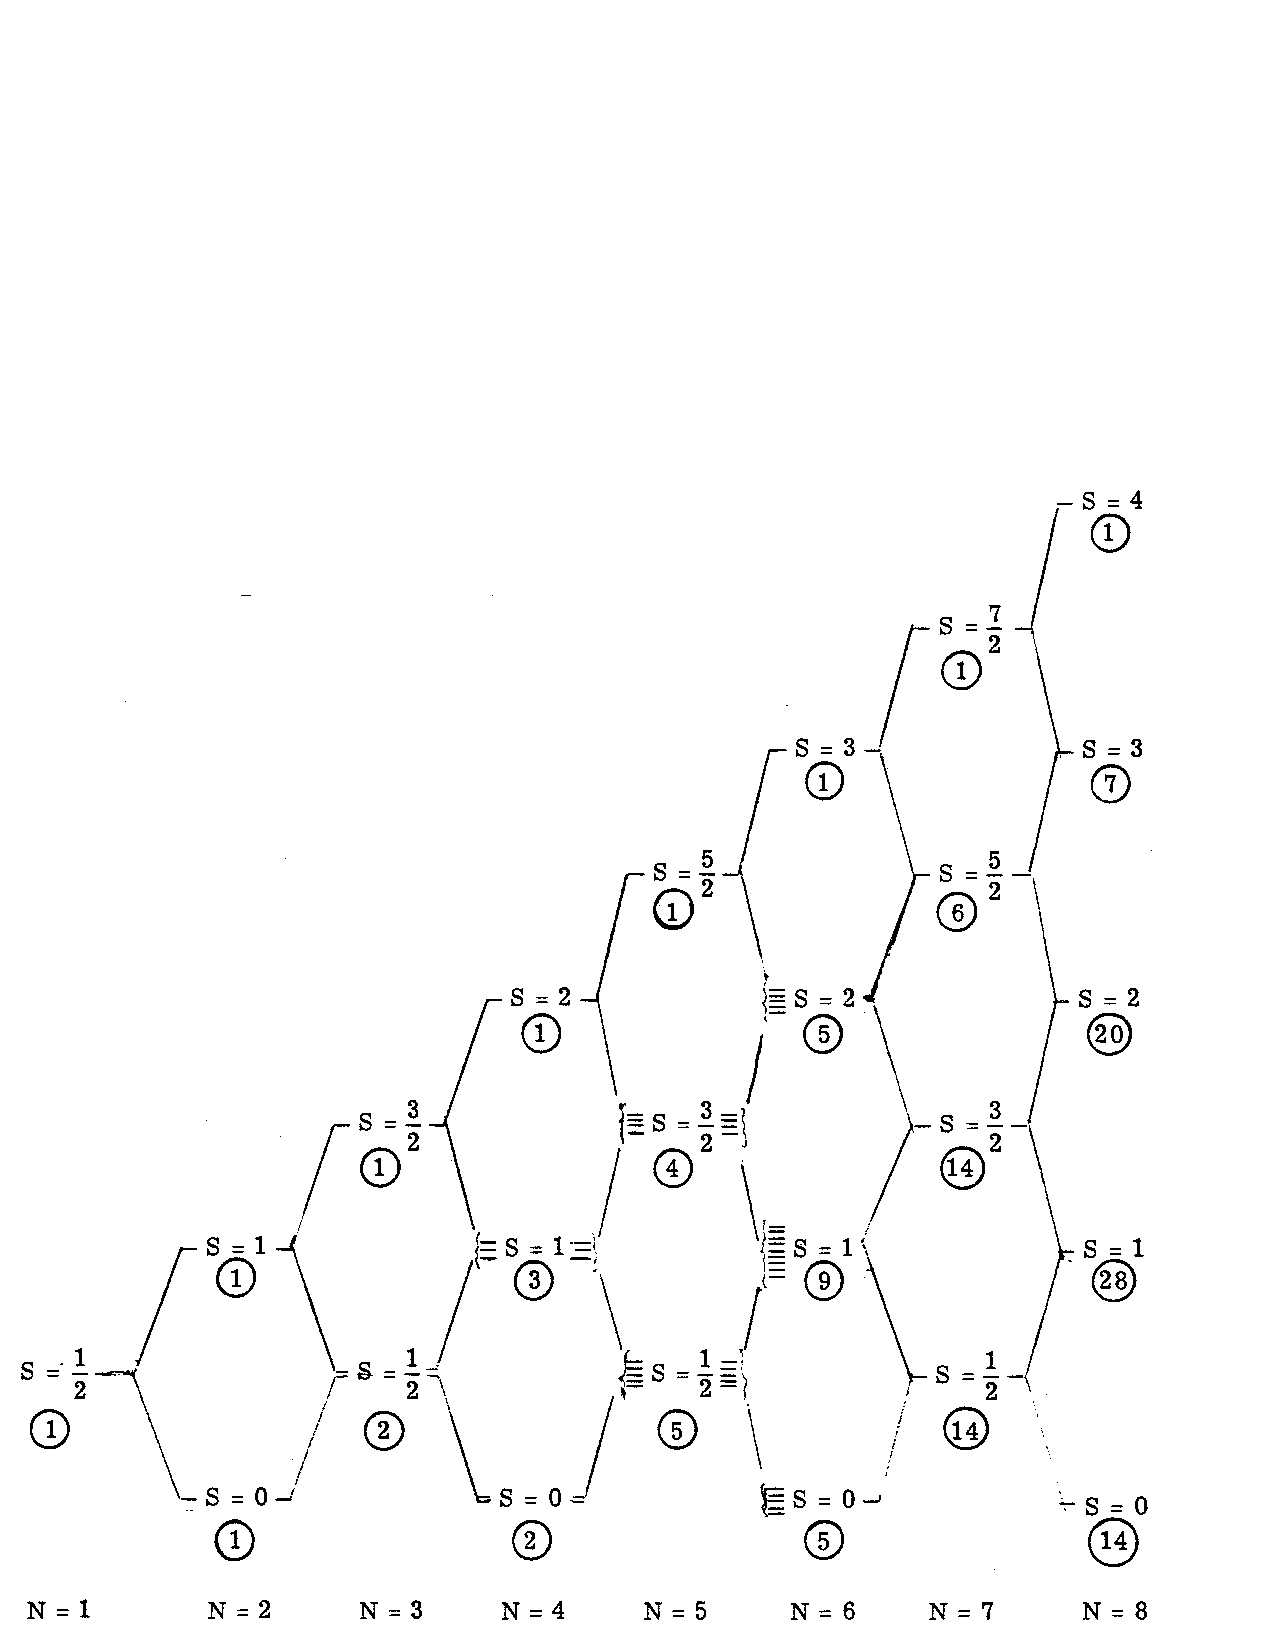
\includegraphics[scale=0.75]{fig4-8}
\caption{Branching diagram for combining electron spins.  The 
number of electrons is indicated by N and the number of independent 
sets of spin states of ech spin S is indicted by the encircled number 
lying below the spin value.}
\label{fig4-02}
\end{figure}


This suggests an inductive procedure for building up the spin 
eigenfunctions $\chi^N_{SM}$ for an arbitrary $N$.  We take a spin 
eigenfunction $\chi^N_{SS}$ and combine it with either $\alpha (N+1)$ 
or $\beta (N+1)$ to obtain
\begin{equation}
\chi^N_{SS} \left( 1 \cdots N \right) \alpha \left( N + 1 \right)
\end{equation}
and
\begin{equation}
\chi^N_{SS} \left( 1 \cdots N \right) \beta \left( N + 1 \right) .
\end{equation}
Partitioning the raising operator ${\hat S}^+_{N+1}$ for $N + 1$ 
electrons into the ${\hat S}^+_N$ for the first $N$ electrons, plus 
${\hat s}^+ (N+1)$, we see that
\begin{equation}
{\hat S}^+_{N+1} \left[ \chi^N_{SS} \alpha \left( N + 1 \right) 
\right] = \left[ {\hat S}^+_N \chi^N_{SS} \right] \alpha + 
\chi^N_{SS} \left[ {\hat s}^+_{(N+1)} \alpha \right] = 0
\end{equation}
and
\begin{equation}
{\hat S}_z \left[ \chi^N_{SS} \alpha \left( N + 1 \right) \right] = 
S + {1 \over 2}.
\end{equation}
Thus,
\begin{equation}
\chi^{N+1}_{S+{1 \over 2},S+{1 \over 2}} = \chi^N_S \alpha 
\left( N + 1 \right) 
\label{chap4app-eqno18}
\end{equation}
is a spin eigenfunction with spin $S + 1/2$.

The function
\begin{equation}
\chi^N_{SS} \beta \left( N + 1 \right)
\end{equation}
has
\begin{equation}
M = S - {1 \over 2} ,
\end{equation}
but it is not an eigenfunction of ${\hat S}^2$.  However, by combining this 
function with the function
\begin{equation}
\chi^N_{S,S-1} \alpha \left( N + 1 \right) = {1 \over 2S} \left( 
{\hat S}^-_N \chi^N_{S,S} \right) \alpha \left( N + 1 \right)
\end{equation}
we can get an eigenfunction of ${\hat S}^2$.  Thus,
\begin{equation}
{\hat S}^+ \left[ \chi^N_{SS} \beta \left( N + 1 \right) - 
\chi^N_{S,S-1} \alpha \left( N + 1 \right) \right] = \chi^N_{SS} 
\alpha \left( N + 1 \right) - \chi^N_{S,S} \alpha \left( N + 1 \right) = 0
\end{equation}
and
\begin{equation}
\chi^{N+1}_{S-{1 \over 2},S-{1 \over 2}} = \chi^N_{S,S} \beta \left( 
N = 1 \right) - {1 \over 2S} \left( S^-_N \chi^N_{S,S} \right) 
\alpha \left( N + 1 \right)
\label{chap4app-eqno19}
\end{equation}
is an eigenfunction of ${\hat S}^2$ corresponding to $S - 1/2$.

Using (\ref{chap4app-eqno18}) and (\ref{chap4app-eqno19})
successively, following any pathway in Figure \ref{fig4-02}, we can
generate spin eigenfunctions of arbitrary $N$ and $S$, assuming we
have sufficient patience.  A following section contains a tabulation
of all spin eigenfunctions up through $N = 6$, generated by a computer
program.  Note, the tableaux have the rows and columns interchanged as
compared to those in this section.

For example, application of (\ref{chap4app-eqno18}) to the $S = 0$
state of (\ref{chap4app-eqno13}) leads to the $S = 1/2$ state of
(\ref{chap4app-eqno16}), while application of (\ref{chap4app-eqno19})
to the $S = 1$ states of (\ref{chap4app-eqno14}) to the $S = 1/2$
state of (\ref{chap4app-eqno17}).

As another example, application of (\ref{chap4app-eqno19}) to the $S =
1/2$ states of (\ref{chap4app-eqno16}) and (\ref{chap4app-eqno17})
lead to the $S = 0$ states of $N = 4$,
\begin{equation}
\chi^{(1)}_{00} = {1 \over 2} \left( \alpha \beta - \beta \alpha 
\right) \left( \alpha \beta - \beta \alpha \right) =
\label{chap4app-eqno20}
\end{equation}
\begin{equation}
\begin{tabular}{l}
\fbox{1}\fbox{3}\\
\fbox{2}\fbox{4}
\end{tabular}
\end{equation}
and
\begin{equation}
\chi^{(2)}_{00} = {1 \over \sqrt{3}} \left[ \alpha \alpha \beta 
\beta + \beta \beta \alpha \alpha - {1 \over 2} \left( \alpha \beta + 
\beta \alpha \right) \left( \alpha \beta + \beta \alpha \right) \right] 
=
\label{chap4app-eqno21}
\end{equation}
\begin{equation}
\begin{tabular}{l}
\fbox{1}\fbox{2}\\
\fbox{3}\fbox{4}
\end{tabular}
\end{equation}
\noindent
There are a number of separate spin eigenfunctions $\chi^N_{S,S}$ for
most cases, and the above inductive procedure for obtaining these
eigenstates leads to a particular sequence.  Always starting with the
lowest $S$ for a given $N$, we number the state for $N + 1$ and any
given $S^{\prime}$ in the order in which they are constructed, for a
given $S^{\prime}$.  This has already been done in
(\ref{chap4app-eqno16}) and (\ref{chap4app-eqno17}), and in
(\ref{chap4app-eqno20}) and (\ref{chap4app-eqno21}).  In general, we
will refer to this first, second, etc., spin eigenfunctions of a given
spin $S$ as $Y1$, $Y2$, etc., in honor of the English clergyman and
mathematician Young$^1$ and the Japanese physicist Yamanouchi,$^2$ who
laid the mathematical foundations for this particular set of spin
eigenfunctions.$^3$

% Removed subsubsection on VB Spin Eigenfunctions goes here

\subsubsection{Tabulation of Spin Eigenfunctions}

Here we list all spin eigenfunctions for up through six 
electrons.$^4$  In each case, only the $M_S = S$ component is given.  
A spin term of 110101 implies $\alpha \alpha \beta \alpha \beta 
\alpha$.  The tableau, e.g.,
\begin{equation}
\begin{tabular}{l}
\fbox{1}\fbox{2} \\
\fbox{3} \\
\fbox{4}
\end{tabular}
\end{equation}

\noindent
associated with each spin eigenfunction, is in the form appropriate 
for the spatial wavefunction corresponding to the particular spin 
function, through the Pauli principle.  Thus, compared to the diagrams 
of the earlier sections, row and columns are interchanged.

The Caltech programs use slightly different sign conventions.  For 
three electrons, it is $-Y1$ for doublet.  For four electrons, it is 
$-Y1$ for singlet and $-Y2$ for triplet.  For five electrons, it is 
$-Y1$ and $-Y4$ for doublet.  And, for six
electrons, it is $-Y1$ and $-Y4$ for singlet, and $-Y1$,$ -Y4$, $-Y6$, 
and $-Y8$ for triplet.  These spin eigenfunctions were generated by 
the MQM program SEFGEN, MQM number 26, written by G. Levin and F. 
W. Bobrowicz.  The following listing has been taken from that program.

\begin{table}
\caption{Spin-Eigenfunction Listing}
\begin{tabular}{lcrr} \\ \hline
& Normalization & Coefficient &Spin Term\cr
1E Doublet & $1/\sqrt{ 1 }$ & 1 & 1\cr
2E Singlet & $1/\sqrt{ 2 }$ & 1 & 10\cr
& & $-1$ & 01\cr
2E Triplet & $1/\sqrt{ 1 }$ & 1 & 11\cr
3E Doublet Y1 & $1/\sqrt{ 2 }$ & 1 & 010\cr
& & $-1$ & 011\cr
3E Doublet Y2 & $1/\sqrt{6}$ & 2 & 110\cr
& & $-$1 & 011\cr
& & $-$1 & 101\cr
3E Quartet & $1/\sqrt{ 1 }$ & 1 & 111\cr
4E Singlet Y1  & $1/\sqrt{ 4 }$ & 1 & 1010\cr
& & $-1$ & 1001\cr
& & $-1$ & 0110\cr
& & 1 & 0101\cr
4E Singlet Y2 & $1/\sqrt{ 12 }$ & 2 & 1100\cr
& & $-$1 & 0101\cr
& & $-$1 & 1001\cr
& & $-$1 & 1010\cr
& & 2 & 0011\cr
& & $-$1 & 0110\cr
4E Triplet Y1 & $1/\sqrt{ 2 }$ & 1 & 1011\cr
& & $-$1 & 0111\cr
4E Triplet Y2 & $1/\sqrt{ 6 }$ & 2 & 1101\cr
& & $-$1 & 1011\cr
& & $-$1 & 0111\cr
4E Triplet Y3 & $1/\sqrt{ 12 }$ & 3 & 1110\cr
& & $-$1 & 0111\cr
& & $-$1 & 1011\cr
& & $-$1 & 1101\cr
4E Quintet & $1/\sqrt{ 1 }$ & 1 & 1111\cr 
\hline
\end{tabular} 
\end{table}
\begin{table}
\begin{tabular}{lcrr} \\ \hline
& Normalization & Coefficient &Spin Term\cr
5E Doublet Y2 & $1/\sqrt{ 12 }$ & 2 & 11001\cr
& & $-$1 & 01011\cr
& & $-$1 & 10011\cr
& & $-$1 & 10101\cr
& & 2 & 00111\cr
& & $-$1 & 01101\cr
5E Doublet Y3 & $1/\sqrt{ 12 }$ & 2 & 10110\cr
& & $-$1 & 10011\cr
& & $-$1 & 10101\cr
& & $-$2 & 01110\cr
& & 1 & 01011\cr
& & 1 & 01101\cr
5E Doublet Y4 & $1/\sqrt{ 36  }$ & 4 & 11010\cr
& & $-$1 & 01011\cr
& & $-$1 & 10011\cr
& & $-$2 & 11001\cr
& & $-$2 & 10110\cr
& & 2 & 00111\cr
& & 1 & 10101\cr
& & $-$2 & 01110\cr
& & 1 & 01101\cr
5E Doublet Y5 & $1/\sqrt{ 72 }$ & 6 & 11100\cr
& & $-$2 & 01101\cr
& & $-$2 & 10101\cr
& & $-$2 & 11001\cr
& & $-$2 & 01110\cr
& & 2 & 00111\cr
& & 2 & 01011\cr
& & $-$2 & 10110\cr
& & 2 & 10011\cr
& & $-$2 & 11010\cr
\hline
\end{tabular}
\end{table}
\begin{table}
\begin{tabular}{lcrr} \\ \hline
& Normalization & Coefficient &Spin Term\cr
6E Singlet Y1 & $1/\sqrt{ 8 }$ & 1 & 101010\cr
5E Quartet Y1 & $1/\sqrt{ 2 }$ & 1 & 10111\cr
& & $-$1 & 01111\cr
5E Quartet Y2 & $1/\sqrt{ 6 }$ & 2 & 11011\cr
& & $-$1 & 10111\cr
& & $-$1 & 01111\cr
5E Quartet Y3 & $1/\sqrt{ 12 }$ & 3 & 11101\cr
& & $-$1 & 01111\cr
& & $-$1 & 10111\cr
& & $-$1 & 11011\cr
5E Quartet Y4 & $1/\sqrt{ 20 }$ & 4 & 11110\cr
& & $-$1 & 01111\cr
& & $-$1 & 10111\cr
& & $-$1 & 11011\cr
& & $-$1 & 11101\cr
5E Sextet & $1/\sqrt{ 1 }$ & 1 & 11111\cr
& & $-$1 & 101001\cr
& & $-$1 & 100110\cr
& & 1 & 100101\cr
& & $-$1 & 011010\cr
& & 1 & 011001\cr
& & 1 & 010110\cr
& & $-$1 & 010101\cr
6E Singlet Y2 & $1/\sqrt{ 24 }$ & 2 & 110010\cr
& & $-$2 & 110001\cr
& & $-$1 & 010110\cr
& & 1 & 010101\cr
& & $-$1 & 100110\cr
& & 1 & 100101\cr
& & $-$1 & 101010\cr
& & 1 & 101001\cr
& & 2 & 001110\cr
& & $-$2 & 001101\cr
& & $-$1 & 011010\cr
& & 1 & 011001\cr
\hline
\end{tabular}
\end{table}
\begin{table}
\begin{tabular}{lcrr} \\ \hline
& Normalization & Coefficient &Spin Term\cr
6E Singlet Y3 & $1/\sqrt{ 24 }$ & 2 & 101100\cr
& & $-$1 & 100101\cr
& & $-$1 & 101001\cr
& & $-$1 & 100110\cr
& & 2 & 100011\cr
& & $-$1 & 101010\cr
& & $-$2 & 011100\cr
& & 1 & 010101\cr
& & 1 & 011001\cr
& & 1 & 010110\cr
& & $-$2 & 010011\cr
& & 1 & 011010\cr
6E Singlet Y1 & $1/\sqrt{ 8 }$ & 1 & 101010\cr
6E Singlet Y4 & $1/\sqrt{ 72 }$ & 4 & 110100\cr
& & $-$1 & 010101\cr
& & $-$1 & 100101\cr
& & $-$2 & 110001\cr
& & $-$1 & 010110\cr
& & 2 & 010011\cr
& & $-$1 & 100110\cr
& & 2 & 100011\cr
& & $-$2 & 110010\cr
& & $-$2 & 101100\cr
& & 2 & 001101\cr
& & 1 & 101001\cr
& & 2 & 001110\cr
& & $-$4 & 001011\cr
& & 1 & 101010\cr
& & $-$2 & 011100\cr
& & 1 & 011001\cr
& & 1 & 011010\cr
& & 2 & 001011\cr
& & 2 & 010011\cr
& & $-$2 & 101010\cr
& & 2 & 100011\cr
& & $-$2 & 110010\cr
& & $-$2 & 011100\cr
& & 1 & 011001\cr
& & 1 & 011010\cr
\hline
\end{tabular}
\end{table}
\begin{table}
\begin{tabular}{lcrr} \\ \hline
& Normalization & Coefficient &Spin Term\cr
6E Singlet Y5 & $1/\sqrt{ 144 }$ & 6 & 111000\cr
& & $-$2 & 011001\cr
& & $-$2 & 101001\cr
& & $-$2 & 110001\cr
& & $-$2 & 011010\cr
& & 2 & 001011\cr
& & 2 & 010011\cr
& & $-$2 & 101010\cr
& & 2 & 100011\cr
& & $-$2 & 110010\cr
& & $-$2 & 011100\cr
& & 2 & 001101\cr
& & 2 & 010101\cr
& & 2 & 001110\cr
& & $-$6 & 000111\cr
& & 2 & 010110\cr
& & $-$2 & 101100\cr
& & 2 & 100101\cr
& & 2 & 100110\cr
& & $-$2 & 110100\cr
6E Singlet Y1 & $1/\sqrt{ 8 }$ & 1 & 101010\cr
6E Triplet YI & $1/\sqrt{ 4 }$ & 1 & 101011\cr
& & $-$1 & 100111\cr
& & $-$1 & 011011\cr
& & 1 & 010111\cr
6E Triplet Y2 & $1/\sqrt{ 12 }$ & 2 & 110011\cr
& & $-$1 & 010111\cr
& & $-$1 & 100111\cr
& & $-$1 & 101011\cr
& & 2 & 001111\cr
& & $-$1 & 011011\cr
\hline
\end{tabular}
\end{table}
\begin{table}
\begin{tabular}{lcrr} \\ \hline
& Normalization & Coefficient &Spin Term\cr
6E Triplet Y3 & $1/\sqrt{ 12 }$ & 2 & 101101\cr
& & $-$1 & 100111\cr
& & $-$1 & 101011\cr
& & $-$2 & 011101\cr
& & 1 & 010111\cr
& & 1 & 011011\cr
6E Triplet Y4 & $1/\sqrt{ 36 }$ & 4 & 110101\cr
& & $-$1 & 010111\cr
& & $-$1 & 100111\cr
& & $-$2 & 110011\cr
& & $-$2 & 101101\cr
& & 2 & 001111\cr
& & 1 & 101011\cr
& & $-$2 & 011101\cr
& & 1 & 011011\cr
6E Triplet Y5 & $1/\sqrt{ 72 }$ & 6 & 111001\cr
& & $-$2 & 011011\cr
& & $-$2 & 101011\cr
& & $-$2 & 110011\cr
& & $-$2 & 011101\cr
& & 2 & 001111\cr
& & 2 & 010111\cr
& & $-$2 & 101101\cr
& & 2 & 100111\cr
& & $-$2 & 110101\cr
6E Triplet Y6 & $1/\sqrt{ 24 }$ & 3 & 101110\cr
& & $-$1 & 100111\cr
& & $-$1 & 101011\cr
& & $-$1 & 101101\cr
& & $-$3 & 011110\cr
& & 1 & 010111\cr
& & 1 & 011011\cr
& & 1 & 011101\cr
\hline
\end{tabular}
\end{table}
\begin{table}
\begin{tabular}{lcrr} \\ \hline
& Normalization & Coefficient &Spin Term\cr
6E Triplet Y7 & $1/\sqrt{ 72 }$ & 6 & 110110\cr
& & $-$1 & 010111\cr
& & $-$1 & 100111\cr
& & $-$2 & 110011\cr
& & $-$2 & 110101\cr
& & $-$3 & 101110\cr
& & 2 & 001111\cr
& & 1 & 101011\cr
& & 1 & 101101\cr
& & $-$3 & 011110\cr
& & 1 & 011011\cr
& & 1 & 011101\cr
6E Singlet Y8 & $1/\sqrt{ 144 }$ & 9 & 111010\cr
& & $-$2 & 011011\cr
& & $-$2 & 101011\cr
& & $-$2 & 110011\cr
& & $-$3 & 111001\cr
& & $-$3 & 011110\cr
& & 2 & 001111\cr
& & 2 & 010111\cr
& & 1 & 011101\cr
& & $-$3 & 101110\cr
& & 2 & 100111\cr
& & 1 & 101101\cr
& & $-$3 & 110110\cr
& & 1 & 110101\cr
6E Triplet Y9 & $1/\sqrt{ 240 }$ & 12 & 111100\cr
& & $-$3 & 011101\cr
& & $-$3 & 101101\cr
& & $-$3 & 110101\cr
& & $-$3 & 111001\cr
& & $-$3 & 011110\cr
& & 2 & 001111\cr
& & 2 & 010111\cr
& & 2 & 011011\cr
& & $-$3 & 101110\cr
& & 2 & 100111\cr
& & 2 & 101011\cr
& & $-$3 & 110110\cr
& & 2 & 110011\cr
& & $-$3 & 111010\cr
\hline
\end{tabular}
\end{table}
\begin{table}
\begin{tabular}{lcrr} \\ \hline
& Normalization & Coefficient &Spin Term\cr
6E Quintet Yl & $1/\sqrt{ 2 }$ & 1 & 101111\cr
& & $-$1 & 011111\cr
6E Quintet Y2 & $1/\sqrt{ 6 }$ & 2 & 110111\cr
& & $-$1 & 101111\cr
& & $-$1 & 011111\cr
6E Quintet Y3 & $1/\sqrt{ 12 }$ & 3 & 111011\cr
& & $-$1 & 011111\cr
& & $-$1 & 101111\cr
& & $-$1 & 101111\cr
& & $-$1 & 110111\cr
6E Quintet Y4 & $1/\sqrt{ 20 }$ & 4 & 111101\cr
& & $-$1 & 011111\cr
& & $-$1 & 101111\cr
& & $-$1 & 110111\cr
& & $-$1 & 111011\cr
6E Quintet Y5 & $1/\sqrt{ 30 }$ & 5 & 111110\cr
& & $-$1 & 011111\cr
& & $-$1 & 101111\cr
& & $-$1 & 110111\cr
& & $-$1 & 111011\cr
& & $-$1 & 111101\cr
6E Septet & $1/\sqrt{ 1 }$ & 1 & 111111\cr \hline
\end{tabular}
\end{table}

\subsection{Historical Development}
\label{chap4-app-d}

In this section, we will provide some of the historical development.  From 
these developments, two very important postulates of quantum mechanics, 
neither of which has an analog in the classical description of electrons, 
will be shown.  The first, is the idea that an electron has an 
internal quantum number called the spin.  The second, in a simplified 
form referred to as the Pauli exclusion principle, is that only one 
electron can have the same set of quantum number, including spin.  
The basic character and properties of molecules are most profoundly 
affected by the combination of the Pauli principle with electron spin.


\subsubsection{Effect of Magnetic Fields}

So far, in this course, we have considered the electron to be point particle
having mass $m$ and charge $-e$.  Thus, we described the electron 
wavefunction as $\varphi ( {\bf r} ) = \varphi ( x , y , z )$
presuming that only the position of the electron need be given.  This is, of
course, an approximation.  We can expect that there must be some sort of 
internal structure for the electron.  However, since the size of an electron 
is about 10$^{-16}$ cm, while the size of the hydrogen
atom is about $10^{-8}$ cm, we would expect that the internal 
structure of the electron would be of no importance to us.  In fact, this 
is quite far from the truth.  The internal structure of the electron plays 
a very important, although indirect, role in chemistry.

\subsubsection{Effect of Magnetic Fields}

The effect of magnetic fields on atomic spectral lines is meant only 
to provide background on the hypothesis of electron spin. The student 
is not responsible for this material.

Classically, an electron moving in a magnetic field {\bf B} 
experiences a force
\begin{equation}
{\bf F}_B = - e ( {\bf v} \times {\bf B} ) 
\end{equation}
called the Lorentz force.  For a uniform $B$, this force, being 
perpendicular to {\bf v} and {\bf B}, leads to a circular orbit of radius 
$R$, where the radius is determined by
\begin{equation}
{mv^2 \over R} = evB
\end{equation}
or
\begin{equation}
v = \left( {e \over m} B \right) R .
\end{equation}
For distances far from this current loop, the magnetic field due to 
this electron motion, is given by
\begin{equation}
{\bf B} = {\mu \over r^3} ,
\end{equation}
where
\begin{equation}
\mu = i A = \left( {e \omega \over 2 \pi c} \right) \left( \pi R^2 
\right) = - \left( {e \over 2c} \right) \omega R^2
\end{equation}
here $i$ is the current in the loop, $A$ is the area of the loop, and 
the $e/c$ is needed to correctly convert units from electrostatic unit 
of charge, and $\omega$ is the angular velocity
\begin{equation}
\omega = {v \over R} .
\end{equation}
Since the angular momentum is
\begin{equation}
l = mvR = m \omega R^2 ,
\end{equation}
we see that
\begin{equation}
\mu = - \left( {e \over 2mc} \right) {\bf l} = - \mu_B {\bf l} 
,
\label{chap4app-eqno27}
\end{equation}
where $\mu_B= e/2mc$ is called the Bohr magneton.

For a state with angular momentum $l$, the component of angular momentum 
along some axis is
\begin{equation}
l_z = \hbar m_l ,
\end{equation}
where $m_l = l , l - 1 , \cdots , -l$.  The magnetic moment along this 
axis is
\begin{equation}
\mu_z = - \left( \hbar \mu_B \right) m_l ,
\end{equation}
leading to $2l + 1$ different magnetic moments.  Now consider an 
external magnetic field along the z axis, $B$. The interaction energy is
\begin{equation}
\Delta E_{m_l} = \mu \cdot B = - \left( {e \hbar B \over 2mc} \right) 
m_l .
\end{equation}
Thus, the $2l + 1$ states with the same total $l$, which are degenerate 
in the absence of a magnetic field, are split by the magnetic field 
into $2l + 1$ states having different energy.  Hence, in a magnetic 
field, the absorption or emission lines corresponding to a transition 
between the $1s$ and $2p$ states of hydrogen, should be
split into three lines, a multiplet, corresponding to the three 
values of $m_l$ for the $2p$ states.

In fact, experimentally one observed two sets of lines, one 
corresponding to $m_l = 2, 2/3, -2/3 , -2$, and the other to $m_l = 1/3, 
-1/3$.  Land\'e, in 1921 and 1923, showed that
the multiplets observed with magentic fields could all be expressed as
\begin{equation}
E ( m_j ) = E_j - \left( {e \hbar B \over 2mc} \right) gm_j ,
\end{equation}
where $g$ has the form
\begin{equation}
g = 1 + {J(J+1) + S(S+1) - L(L+1) \over 2J(J+1}
\label{chap4app-eqno28}
\end{equation}   
where $L$, $S$, and $J$ are integers, or half integers, and $m_j$ 
ranges in integer increments from $+J$ to $-J$, inclusive.  For one-electron 
atoms, such as H and Na, the value of $S$ is always one half.

Uhlenbeck and Goudsmit, in 1925, showed that the Land\'e formula could be
derived by assuming that electrons have an intrinsic angular momentum 
{\bf s} and an associated magnetic moment $\mu_s$ where
\begin{equation}
\mu_s = - \left( {e \over mc} \right) {\bf s}
\label{chap4app-eqno29}
\end{equation}
that is, the proportionality constant is twice the value obtained in
(\ref{chap4app-eqno17}), i.e., $g = 2$ in (\ref{chap4app-eqno28}), and
where the allowed values of $s$ parallel to the magnetic field are
$s_z = \hbar m_s$ with $m_s = \pm 1/2$.  For a one-electron atom, the
resulting values of $J$ are then $J = L + 1/2$ and $J = L - 1/2$, so
that $L = 1$ leads to $J = 3/2$, with four values of $M_J$, and $J =
1/2$, with two values of $M_J$.  This led to an excellent
rationalization of the observed multiplet structures of atom, and
provided convincing evidence of the existence of electron spin.

\subsubsection{The Dirac Equation}

Dirac, in about 1930, reformulated the Schr\"odinger equation
\begin{equation}
\left[ - {1 \over 2m} \nabla^2 + V (R) \right] \psi = i \hbar 
{\partial \psi \over \partial t}
\end{equation}
to make it relativistically correct.  He found that this relativistic
formulation lead to the possibility of an angular momentum associated
with the internal coordinates with the smallest nonzero value being
1/2.  This leads to two possible projections, $m_s = \pm 1/2$.  He
found, directly from relativist quantum mechanics, that the magnetic
moment $\mu$ associated with the spin angular momentum {\bf s} is
given by (\ref{chap4app-eqno29}), just as assumed by Uhlenbeck and
Goudsmit. The fact that relativistic quantum mechanics leads directly
to $g = 2$ for an electron, was considered quite a success and
provided a firm foundation for the concept of electron spin.  It is
known now, that $g = 2.00231931$.  However, the deviation from $g = 2$
is understood as arising from quantum effects involving the radiation
field.

\subsubsection{The Pauli Exclusion Principle}

Pauli introduced new quantum numbers $m_s = \pm 1/2$ in the
exclusion principle he formulated in explaining the periodic table.  
Thus the existence of electron spin angular momenta, having quantum 
number $m_s = \pm 1/2$, provides a physical basis for Pauli's hypothesis.

On the basis of the Sommerfeld-Bohr model of the atom, there were two quantum
numbers $n$ and $k$, written as $n_k$, describing the major and minor axes 
of the elliptical orbitals. The energy depended only on $n$, and $k$ 
ranged from $l$ to $n$, in integer increments.  Small $k$ orbits 
penetrated the core, more than large $k$, so that for many-electron 
atoms $n_1$ is lowest and $n_n$ is higher in energy.  Indeed, we can 
think of $k$ as analogous to $l + 1$, although $k$ did not have the 
significance of an angular momentum.  Initially,
Bohr thought that many-electron atoms had all the electrons in the 
$l_1$ type orbits, but he soon realized, from experimental observations, 
that the stable configurations for most atoms must have some electrons 
in higher energy orbits.  There were, of course, an
infinite number of possible orbits for even the $l_1$ level, so it was 
assumed that particular arrangements of orbits were particularly stable so 
that additional electrons would be force to go into higher
orbits.  Since the inert gases must have such stable configurations, Bohr by
1922 had concluded that the inert gas configurations are as shown in
Table 
\ref{chap4app-table1}.

The major difficulty here was that no one knew what lead to the 
closing of the electronic shells.  Why 2 for $1_1$, but 4 for $2_1$, and 
two dfferent limits for $3_1$?  In 1924, Pauli was trying to understand the 
doublet nature of the Na spectrum.  Noticing that the
Land\'e scheme led to half-integral quantum number for Na, Pauli suggested 
that it was due to a new quantum theoretical property of the electron, 
that he called, classically nondescribable two-valuedness.  At the time, 
the doublet spectrum was thought to be due to a nonvanishing angular 
momentum of the atomic core.  We would now call this spin, with 
$m_s = \pm 1/2$ as the two values.

In 1925, Pauli suggested his exclusion principle.  It is that now two 
electrons can have the same set of quantum numbers, including $m_s$.  
This, then, provided the mechanism for closing the shells, and hence, for 
understanding the periodic table.  To do
this correctly also required the quantum mechanics of Schr\"odinger, in 1926, 
which leads to three spatial quantum number $nlm_l$ supplemented by 
$m_s$.  Assuming a proper sequence of $nl$ shells, these ideas led to 
the Aufbau principle providing the explanation of the periodic table, 
and also, a systematic understanding of the spectrum of the various 
atoms.

\subsubsection{The Aufbau Principle}

The first ionization potentials of the first twenty elements, are
listed in Table \ref{chap4app-table2}.  The striking feature is
sequences of continuously increasing ionization potentials separated
by breaks after He, Ne and Ar, at which the ionization potentials
decrease drastically.

In Section \ref{chap4-app-b} we include a simple calculation
indicating that describing He as having two electrons in an optimum
1s-like orbital, leads to an ionization potential of 23.1 eV, in good
agreement with experiment, while describing Li as having three
electrons in an optimum $1s$-like orbitals, leads to an ionization
potential of 377 eV, in gross disagreement with experiment.  On the
other hand, if we arbitrarily restrict each spatial orbital to
contain, at most, two electrons, then Li must have the third electron
in a loosely bound 2$s$ orbital, in agreement with the small
ionization potential of Li.  Assuming the atomic orbitals to have
energies in the order 1$s$, 2$s$, 2$p$, 3$s$, 3$p$, 4$s$, 3$d$, and
4$p$, with big jumps to energy after 1$s$, after 2$p$, after 3$p$,
etc., leads to the configurations indicated in Table
\ref{chap4app-table3}, and provides and explanation of the pattern of
ionization potentials in Table \ref{chap4app-table2}.  This simple
approach, of describing the states of atoms, is called the Aufbau
principle.  Although not exact, the principle has been extremely
useful in understanding the periodic table and in explaining atomic
spectroscopy.  These successes can be taken as strong empirical
evidence, in favor of the hypotheses of the Pauli principle and of
electron spin.


\begin{table}
\caption{}
\label{chap4app-table1}
\begin{tabular}{ccccccc}\\ \hline
& He & Ne & Ar & Kr & Xe & Rd\cr
\noalign{\medskip\hrule\medskip}
$1_1$ & 2 & 2 & 2 & 2 & 2 & 2\cr
$2_1$ & & 4 & 4 & 4 & 4 & 4\cr
$2_2$ & & 4 & 4 & 4 & 4 & 4\cr
$3_1$ & & & 4 & 6 & 6 & 6\cr
$3_2$ & & & 4 & 6 & 6 & 6\cr
$3_3$ & & & & 6 & 6 & 6\cr
$4_1$ & & & & 4 & 6 & 8\cr
$4_2$ & & & & 4 & 6 & 8\cr
$4_3$ & & & & & - & 8\cr
$4_4$ & & & & & - & 8\cr
$5_1$ & & & & & 4 & 6\cr
$5_2$ & & & & & & 6\cr
$5_3$ & & & & & & 6\cr
$5_4$ & & & & & & -\cr
$5_5$ & & & & & & -\cr
$6_1$ & & & & & & 4\cr
$6_2$ & & & & & & 4\cr
\end{tabular}
\end{table}

\begin{table}
\caption{First IP for atoms.}
\label{chap4app-table2}
\begin{tabular}{cc}\\ \hline
& IP (eV)\cr
H & 13.595\cr
He & 24.580\cr
Li & 5.390\cr
Be & 9.320\cr
B &  8.296\cr
C &  11.264\cr
N &  14.54\cr
0 &  13.614\cr
F &  17.42\cr
Ne & 21.559\cr
Na & 5.138\cr
Mg & 7.644\cr
Al & 5.984\cr
Si & 8.149\cr
P &  11.0\cr
S &  10.357\cr
Cl & 13.01\cr
Ar & 15.755\cr
K &   4.339\cr
Ca & 6.111\cr
\end{tabular}
\end{table}

\begin{table}
\caption{Aufbau principle for atoms.}
\label{chap4app-table3}
\begin{tabular}{ccccccccc} \\ \hline
& H & He & Li & Be & B & F & Ne & Na\cr
4p\cr
3d\cr
4s\cr
3p\cr
3s & & & & & & & & x\cr
2p & & & & & x & xxxxx & xxxxxx & xxxxxx\cr
2s & & & x & xx & xx & xx & xx & xx\cr
1s & x & xx & xx & xx & xx & xx & xx & xx\cr
\end{tabular}
\end{table}